%%%%% Please set the path to 'beamer' directory in your environment %%%%%
\newcommand{\beamerDir}[0]{/mnt/c/Users/atsushi/Documents/workspace/env/Beamer/beamer/beamer/}


%%%%% Load setting %%%%%
\documentclass[aspectratio=169, dvipdfmx, 12pt, compress]{beamer}% dvipdfmxしたい

%%%%% Packages %%%%%
\usepackage{bxdpx-beamer}% dvipdfmxなので必要
\usepackage{pxjahyper}% 日本語で'しおり'したい
\usepackage{tikz}
\usepackage{tcolorbox}
\usetikzlibrary{shapes}
\usepackage{xcolor}
\usepackage[absolute,overlay]{textpos}
\usepackage{adjustbox}
\usepackage{caption}
\usepackage{ifthen}


%%%%% Settings %%%%%
\usetheme[sectionpage=progressbar, subsectionpage=progressbar]{metropolis}
% block style
\metroset{block=fill}
% space between line
\renewcommand{\baselinestretch}{1.3}
% space between item
\newlength{\wideitemsep}
\setlength{\wideitemsep}{0.9\itemsep}
% \addtolength{\wideitemsep}{1.0pt} <- more space
\let\olditem\item
\renewcommand{\item}{\setlength{\itemsep}{\wideitemsep}\olditem}
% frame title
\definecolor{coolblack}{rgb}{0.0, 0.18, 0.39}
\setbeamercolor{frametitle}{bg=coolblack!90,fg=white}
\setbeamerfont{frametitle}{size=\large}
\addtobeamertemplate{frametitle}{}{\vspace{-1em}}
\makeatletter
\setlength{\metropolis@frametitle@padding}{1.4ex}% <- default 2.2 ex
% foot line
\addtobeamertemplate{footline}{}{\vspace{-1em}}
% normal text color
\setbeamercolor{normal text}{fg=black!80}
% progress bar
\definecolor{lightgray}{rgb}{0.83, 0.83, 0.83}
\setbeamercolor{progress bar}{bg=lightgray, fg=coolblack}
\setbeamersize{text margin left=15pt, text margin right=15pt}
% equation font
\usefonttheme{professionalfonts}
% Change standard block width
\addtobeamertemplate{block begin}{%
    \centering
    \begin{columns}\begin{column}{0.9\textwidth}
            \centering
            }{}
            \addtobeamertemplate{block end}{}{\end{column}\end{columns}}
% Change alert block width
\addtobeamertemplate{block alerted begin}{%
    \centering
    \begin{columns}\begin{column}{0.9\textwidth}
            \centering
            }{}
            \addtobeamertemplate{block alerted end}{}{\end{column}\end{columns}}
% Change example block width
\addtobeamertemplate{block example begin}{%
    \centering
    \begin{columns}\begin{column}{0.9\textwidth}
            \centering
            }{}
            \addtobeamertemplate{block example end}{}{\end{column}\end{columns}}
% Itemize color
\setbeamertemplate{itemize item}{\color{black}\scriptsize$\blacksquare$}
\setbeamertemplate{itemize subitem}{\color{black}\scriptsize$-$}
% Simplification  color
\definecolor{cobalt}{rgb}{0.0, 0.28, 0.67}
\setbeamercolor{block title example}{fg=black!80,bg=cobalt!35}
\setbeamercolor{block body example}{fg=black,bg=cobalt!15}
% Definition
\BeforeBeginEnvironment{definition}{
    \setbeamercolor{block title}{use=alerted text, bg=alerted text.fg!70,fg=white}
    \setbeamercolor{block body}{use=alerted text, bg=alerted text.fg!20}
}
\AfterEndEnvironment{definition}{% return to default
    \setbeamercolor{block title}{use=structure,fg=structure.fg,bg=structure.fg!20!bg}
    \setbeamercolor{block body}{parent=normal text,use=block title,bg=block title.bg!50!bg, fg=black}
}
% Theorem
\definecolor{seagreen}{rgb}{0.18, 0.55, 0.34}
\setbeamertemplate{theorems}[numbered]
\BeforeBeginEnvironment{theorem}{
    \setbeamercolor{block title}{fg=black!80,bg=seagreen!40}
    \setbeamercolor{block body}{fg=black,bg=seagreen!15}
}
\AfterEndEnvironment{theorem}{% return to default
    \setbeamercolor{block title}{use=structure,fg=structure.fg,bg=structure.fg!20!bg}
    \setbeamercolor{block body}{parent=normal text,use=block title,bg=block title.bg!50!bg, fg=black}
}
% Lemma
\undef{\lemma}
\newtheorem{lemma}{\translate{Lemma}}
\BeforeBeginEnvironment{lemma}{
    \setbeamercolor{block title}{fg=black!80,bg=seagreen!20}
    \setbeamercolor{block body}{fg=black,bg=seagreen!10}
}
\AfterEndEnvironment{lemma}{% return to default
    \setbeamercolor{block title}{use=structure,fg=structure.fg!80,bg=structure.fg!20!bg}
    \setbeamercolor{block body}{parent=normal text,use=block title,bg=block title.bg!50!bg, fg=black}
}


%%%%% Original Command %%%%%
\newcommand{\subt}[1]{\vspace{-2mm}{\fontsize{10pt}{0cm}\selectfont \textcolor{lightgray}{#1}}\vspace{-1mm}}
\newcommand{\lastpage}[0]{\begin{frame}\begin{textblock*}{1.0\linewidth}(0pt, 50pt)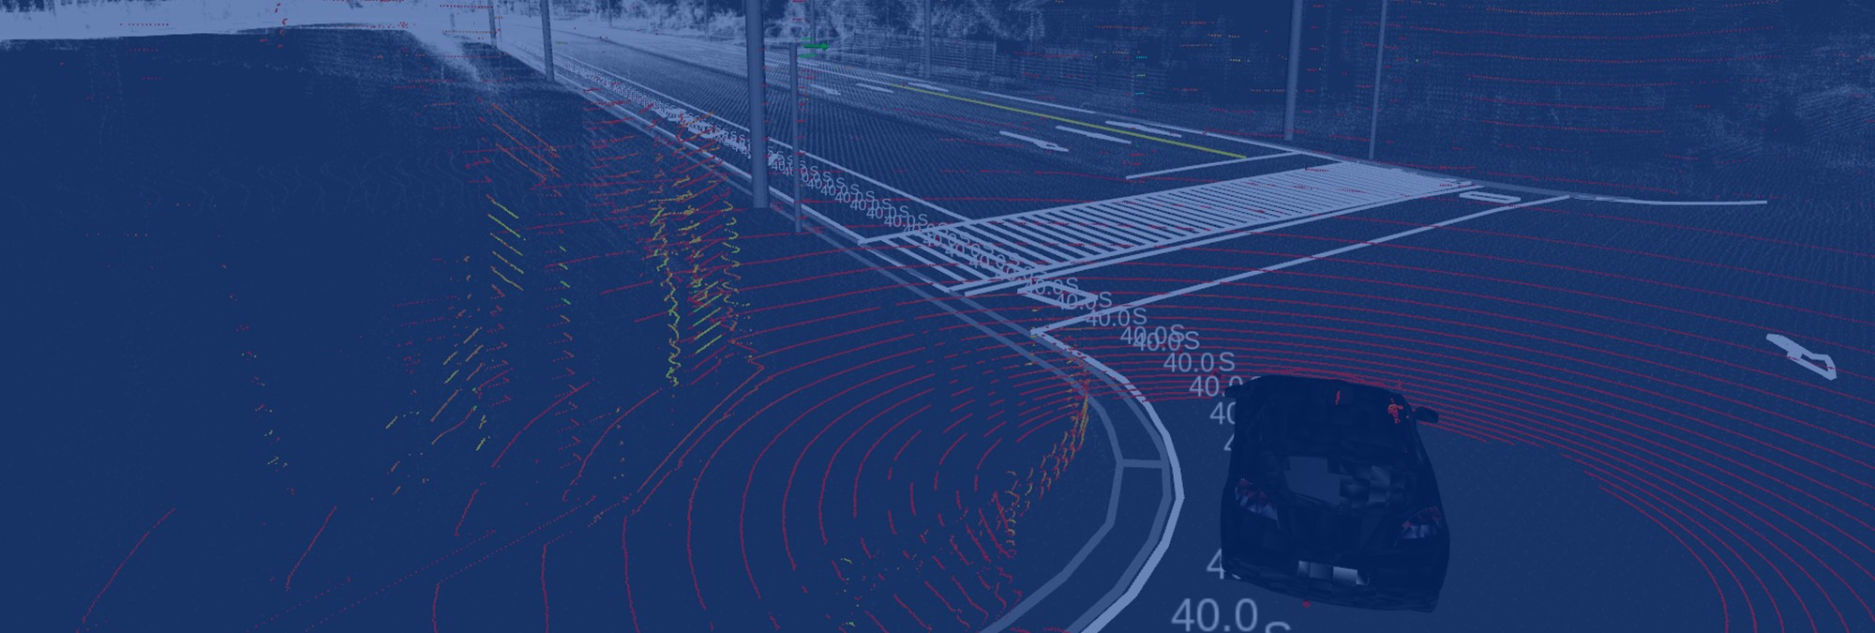
\includegraphics[scale=0.512]{\beamerDir/master_figure/last.pdf}\end{textblock*}\end{frame}}
\newcommand{\todo}[1]{\al{\LARGE\textbf{TODO:} #1}}
\newcommand{\headerheight}[0]{5mm}
\newcommand{\footerheight}[0]{5mm}
\newcommand{\slideheight}[0]{\textheight-\headerheight-\footerheight}
\newcommand{\tabml}[1]{\hspace{-2.1mm}\begin{tabular}{l} #1 \end{tabular}}
\newcommand{\al}[1]{\alert{#1}}
\newcommand{\argempty}[0]{}
\newcommand{\onlyslide}[1]{
    \vspace{\headerheight}
    \begin{minipage}[c][\slideheight][c]{\textwidth}
        #1
    \end{minipage}
}
\newcommand{\onlyimage}[1]{
    \onlyslide{
        \centering
        \begin{columns}
            \begin{column}{\textwidth}
                \centering
                \adjustbox{max width=\textwidth, max height=\slideheight}{
                    \includegraphics{#1}
                }
            \end{column}
        \end{columns}
    }
}
% fit image
\newlength\fitimageht
\newlength\fitotherht
\newsavebox\fitimagebox
\newcommand{\fitimage}[2]{%
    \sbox\fitimagebox{%
        \parbox{\textwidth}{%
            #1\par
        }%
    }%
    \settototalheight{\fitotherht}{%
        \usebox\fitimagebox
    }%
    \setlength\fitimageht{\textheight}%
    \addtolength\fitimageht{-\fitotherht-\headerheight-\footerheight-1\baselineskip}%
    \vspace{\headerheight}
    #1\par
    \centering
    \includegraphics[width=\textwidth,height=\fitimageht,keepaspectratio]{#2}
}
% Simplification
\newcommand{\assume}[1]{
    \begin{exampleblock}{Simplification }
        #1
    \end{exampleblock}
}
% Re-post
\setbeamercolor{RepostBox}{fg=black!50, bg=coolblack!10}
\newcommand{\repost}[1]{
    \vspace{2mm}
    \centering
    \begin{columns}
        \begin{column}{0.86\textwidth}
            \begin{beamercolorbox}[wd=\textwidth, sep=2pt, rounded=true, shadow=true]{RepostBox}
                \begin{tabular}{|p{0.95\textwidth}}
                    {\fontsize{10pt}{10pt}#1}
                \end{tabular}
            \end{beamercolorbox}
        \end{column}
    \end{columns}
}

% equation ballon
\tcbset{
    framebox/.style={
            enhanced,
            boxsep=0pt,       % 箱の上下左右の余白を指定
            colback=white,
            boxrule=1pt,
            colframe=#1
        },
    framebox/.default=red
}
\newcommand{\upbln}[3]{
    \tcboxmath[
        framebox=#2,
        top=0.5ex,bottom=0.5ex,    % 箱の上下の余白を指定
        left=0.5ex,right=0.5ex,    % 箱の左右の余白を指定
        overlay={
                \node[
                    above,
                    rectangle callout,                         % nodeを吹き出しの形に
                    callout absolute pointer={(frame.north)},  % 吹き出しの先端を絶対的に指定
                    fill=#2!20
                ] at ([yshift=2ex]frame.north) {\footnotesize#3};
            }
    ]{#1}
}
\newcommand{\lwbln}[3]{
    \tcboxmath[
        framebox=#2,
        top=0.5ex,bottom=0.5ex,    % 箱の上下の余白を指定
        left=0.5ex,right=0.5ex,    % 箱の左右の余白を指定
        overlay={
                \node[
                    below,
                    rectangle callout,                         % nodeを吹き出しの形に
                    callout absolute pointer={(frame.south)},  % 吹き出しの先端を絶対的に指定
                    fill=#2!20
                ] at ([yshift=-2ex]frame.south) {\footnotesize#3};
            }
    ]{#1}
}
\tcbuselibrary{theorems,skins}



%%%%% Mode %%%%%
% \newcommand{\forme}[1]{#1}
\newcommand{\forme}[1]{}


%%%%% Front Cover %%%%%
\title{PiCAS: New Design of Priority-Driven Chain-Aware Scheduling for ROS2}
\subtitle{IEEE Real-Time and Embedded Technology and Applications Symposium (RTAS), 2021}
\author{矢野 篤志}
\date{\today}
\institute[EMBIV]{EMBIV}
\logo{\begin{textblock*}{0.1\linewidth}(2pt, 237pt)
\includegraphics[scale=0.4]{\beamerDir/master_figure/Emb_logo.pdf}\end{textblock*}}


%%%%% Document Start %%%%%
\begin{document}

\maketitle

% \summary{-5}{2}
% !TeX root = main.tex


\begin{frame}{提案の概要}
    \begin{itemize}
        \item 優先度駆動型スケジューリングによってROSのリアルタイム性能と予測可能性を大幅に改善できることを主張する
        \item 主張を裏付けるために, 優先度駆動型チェーン考慮スケジューリングに関する我々の研究をレビューし, Apex.AI が開発したオープンソースリファレンスシステムを用いた評価を行う
        \item ROS 2のリアルタイム性能を向上させるために不可欠な以下2つの課題を説明する
        \begin{itemize}
            \item マルチスレッドエグゼキュータ設計
            \item アクセラレータサポート
        \end{itemize}
    \end{itemize}
\end{frame}


\begin{frame}{Outline}
    \setbeamertemplate{section in toc}[sections numbered]
    \scriptsize\tableofcontents[hideallsubsections]
\end{frame}

% % !TeX root = main.tex

\section{INTRODUCTION}
\label{sec: introduction}

\begin{frame}{}
    \begin{itemize}
        \item ロボット工学のような, 様々な分野の深い専門知識を必要とする学際的で複雑なアプリケーション領域では, 通常, 全ての, あるいはほとんどのソフトウェアをゼロから書くという選択肢はあり得ない
        \item その代わりに, ロボット工学者は, ROSのような一般的なロボット工学フレームワークで容易に利用できる, 標準機能を提供する既存のサードパーティコンポーネントの統合を採用するのが一般的である
        \item その利点は数多く, 簡単に理解できる
        \item 例えば, 複数の最新パス計画アルゴリズムと3D可視化サポートを備えた完全なナビゲーションスタックがたった1回のダウンロードで手に入るなら, なぜ新しいナビゲーションサブシステムを苦労して開発する必要があるか?
    \end{itemize}
\end{frame}

\begin{frame}{}
    \begin{itemize}
        \item 完全なロボットシステムを構築するためには, 多くの相互作用するコンポーネントを統合する必要がある
        \item ROS開発プロセスの分散型オープンソースの性質により, これらのコンポーネントは通常, 必ずしもお互いを知らない複数の独立したコンポーネント開発者によって分離して開発される
        \item 同様に, システムインテグレータは, アプリケーションおよびミッション固有のロジックと「グルーコード」で展開プラットフォーム上で選択したコンポーネントを構成するが, 通常, それぞれのコンポーネント開発者と密接に連携することはない
    \end{itemize}
\end{frame}

\begin{frame}{}
    \begin{itemize}
        \item コンポーネントの統合を可能な限りシンプルに保つために, ROSはコンポーネントの疎結合を可能にする古典的なトピックベースのpublish/subscribeパラダイムを採用している
        \item 概念的には, 各コンポーネントは, 特定のトピックをsubscribeする多数のコールバックを含む「ブラックボックス」として理解できる
        \item 与えられたトピックに関連するメッセージがpublishされるたびに, 全てのsubscribeコールバックが呼び出され, 何らかの計算を実行し, 次に他のトピックに後続のメッセージをpublishすることができ, これがさらにコールバックをトリガするというように, 繰り返す
    \end{itemize}
\end{frame}

\begin{frame}{}
    \begin{itemize}
        \item インテグレータは, あるコンポーネントの「入力コールバック」を別のコンポーネントの「出力トピック」に接続することによってコンポーネントを構成する
        \item ROSシステムは, このように相互接続されたトピックとコールバックの複雑なネットワークを形成し, データ (環境刺激など) は, イベント駆動型の方法でネットワークを通じてcause-effectチェーンに沿って伝播し, インテグレータが望むように透過的にコンポーネント境界を交差させることができる
    \end{itemize}
\end{frame}

\begin{frame}{}
    \begin{itemize}
        \item このようなcause-effectチェーンの典型的な例として, 進路上の障害物を検知して反応する必要のある移動ロボットのセンシング-計算-行動パイプラインが挙げられる
        \item 例えば, ハードウェアドライバコンポーネントがレーザースキャナから新しいサンプルを取得し (cause) , それが複数のマッピング, 座標変換, パス計画, 車輪制御コンポーネントを経て, 最終的に車輪速度の変化 (effect) をもたらす可能性がある
        \item このようなデータ処理のチェーンにおいて, causeからeffectまでの最大レイテンシ時間は, ロボットが正しく機能するために重要な役割を果たすことは明らかであり, また, 安全性を考慮する上でも重要であることが多い
    \end{itemize}
\end{frame}

\begin{frame}{}
    \begin{itemize}
        \item 重要なのは, システムインテグレータにできるだけ多くの展開の選択肢を残し, コンポーネントの再利用の機会を最大化するために, ROSの実行管理層と基礎となるオペレーティングシステムは, 意図的にコンポーネント開発者に公開されないことである
        \item むしろ, ROSの中心的なコールバック抽象化は, コールバック手続きがいつどのようにスケジュールされるか, コールバックの実行がスレッドまたはプロセスにわたってどのように組織されるか, またはネットワーキング層がメッセージの送受信をどのように処理するかを全く意識せずに, 実行から完了までセマンティクスを持つ単なる手続きである
    \end{itemize}
\end{frame}

\begin{frame}{}
    \begin{itemize}
        \item ROSはオープンソースソフトウェアであるため, 原理的にはシステムの実行と通信の挙動を完全に理解し制御することが可能である
        \item このため, リアルタイムシステムの専門家から見れば, ROSにリアルタイムシステム研究でよく知られた技術を導入することは論理的なステップであるように思える可能性がある
        \item しかし, 一見したところ, これを難しくしているハードルがいくつかある
    \end{itemize}
\end{frame}

\begin{frame}{}
    \begin{itemize}
        \item まず第一に, インテグレータに必要な情報が不足している
        \item ほとんどのリアルタイム分析では, 同時実行タスクの数, それらの起動セマンティクスや機能的相互作用, メッセージの到着パターン, 最悪実行時間など, 多くの低レベルシステムの詳細に関する深い知識が前提となっている
        \item ROSコンポーネントは, この種の情報を提供するマニフェストと一緒に来ることはない
        \item さらに悪いことに, リアルタイム分析は, 欠陥のある情報や不完全な情報にうまく対処できない
        \item モデリング目的でサードパーティコンポーネントを手作業でリバースエンジニアリングしているときに, たった一つのミスや見落としがあれば, その取り組み全体を無条件に無効にしてしまうことになりかねない
    \end{itemize}
\end{frame}

\begin{frame}{}
    \begin{itemize}
        \item 第二に, 必要なシステムの詳細をコンポーネントレベルで静的に決定し, 記述することができない
        \item その理由のひとつは, 多くのロボット工学アルゴリズムが, ユースケースやプラットフォーム固有の側面に依存し, 実行時間や起動パターンが大きく変化するためである
        \item 例えば, ビデオストリーム中の物体を識別し, その軌跡を推測する一般的な物体追跡コンポーネントを考えてみよう (例えば, 隣の車線の車など)
        \item この機能の実行時間は, ビデオストリームのフレームレート, 解像度, コーデック, および特定のトラッキングアルゴリズムに関連する他の様々なパラメータを含む, 様々なパラメータに依存する
        \item これらのパラメータは, 一般的なオブジェクトトラッキングコンポーネントの開発者が前もって知っていたり, 固定されていたりするものではない
    \end{itemize}
\end{frame}

\begin{frame}{}
    \begin{itemize}
        \item このようなユースケース特有の情報は, 特定のロボットを構築するインテグレーターにしか分からない
        \item インテグレーターは, 必ずしもオブジェクトトラッキングやリアルタイムシステムの専門家ではないため, 特定の構成を選択した場合の影響を常に予測できるわけではない
        \item したがって, コンポーネントのリソース要求とリアルタイム動作は, 常に特定の展開で使用するという文脈で評価されなければならない
        \item これは, ROSフレームワークの人気の根底にある「ブラックボックス」コンポーネントのモジュール式再利用と相容れるものではない
    \end{itemize}
\end{frame}

\begin{frame}{}
    \begin{itemize}
        \item 最後に, 仮にインテグレータが各コンポーネントについてそれぞれの専門家と議論し, タイミング分析に必要な全ての詳細を入手できたとしても, 第三の根本的な問題が残る
        \item 多くのコンポーネントのリソース要件と性能特性は, 本質的にロボットの動的環境に依存し, したがって時間とともに変化するため, 静的 (最悪のケース) リソース配置は実行不可能なのである
    \end{itemize}
\end{frame}

\begin{frame}{}
    \begin{itemize}
        \item 例えば, 前述の物体追跡コンポーネントと, ランドマークベースの自己位置特定コンポーネントに依存するロボットを再度考えてみよう
        \item 一方, 人口が少ない田舎町よりも, にぎやかな街中を移動する方が, 物体追跡装置の処理時間はずっと長くなる
        \item 一方, 認識可能なランドマークが多い都市部では, ほぼ一様な風景よりも自己位置推定がはるかに容易である可能性が高い
        \item どちらの状況でも十分なリソースを確保するためには, システムインテグレーターは, 不毛の土地からなる賑やかな都市を想定したシステムを用意しなければならない
    \end{itemize}
\end{frame}

\begin{frame}{}
    \begin{itemize}
        \item ロボット工学では, このような悲観的なシステム設計を行うと, すぐに現実的な限界に直面することになる
        \item その代わりに, 実用的で費用対効果の高いシステムを維持するためには, 各コンポーネントのピーク需要の合計ではなく, 予想されるジョイントリソースのピーク需要に対してプロビジョニングを行う必要がある
    \end{itemize}
\end{frame}

\begin{frame}{貢献する}
    \begin{itemize}
        \item これらの課題を克服するために, 我々は, 実行時に動的にタイミングを考慮した方法でROSシステムをプロビジョニングするための自動レイテンシマネージャを使用することを提案する
        \item 具体的には, ROS Live latency manager (ROSLlama) を紹介する
        \item これは, 重要なcause-effectチェーンに沿ったレイテンシを, 非リアルタイム専門家が使いやすく, かつ設定にあまり手間をかけない方法で, 既存のリアルタイム機構を使用して制御することを可能にする
    \end{itemize}
\end{frame}

\begin{frame}{貢献する}
    \begin{itemize}
        \item ROS-Llamaは, 複雑なシステムパラメータをユーザに要求するのではなく, 実行時に必要なパラメータを自動的に推定し, 状況の変化に応じてスケジューリングパラメータを動的に調整することが可能である
        \item もし, 指定されたレイテンシの目標が全て同時に達成できない場合 (例えば, 不利な環境条件による一時的な過負荷が原因) , ROS-Llamaは制御された緩やかなデグレードプロセスを開始し, システムインテグレーターが純粋に宣言的な方法で (すなわち, cause-effectチェーンがどの部品を通過しているかを理解しなくても) cause-effectチェーンの重要性を特定できるようにする
    \end{itemize}
\end{frame}

\begin{frame}{本論文の貢献}
    \begin{itemize}
        \item  ロボティクス領域における動的レイテンシ管理問題を探求し, 実用的なソリューションが満たさなければならない制約と要件を文書化する (第III章)

        \item  ROSのための最初の自動レイテンシマネージャであるROS-Llamaの設計と実装を紹介する (セクションIV)

        \item 標準的な Linux システム上の ROS コンポーネントを用いて, ROS-Llama が移動ロボットのcause-effectチェーンのレイテンシをうまく制御できることを示す評価について報告する (セクションVI)

    \end{itemize}
\end{frame}

\begin{frame}{}
    \begin{itemize}
        \item ROS-Llamaは, 数年にわたる研究とエンジニアリングの努力の結果であり, その間, 我々は多くの課題や技術的な限界に遭遇した
        \item セクションVIIでは, 以下の点を強調する
              \begin{itemize}
                  \item  ROS-Llamaをより効果的かつ正確にするための分析改善の機会
                  \item  ROSとLinuxのプラットフォームには, システムのさらなる改良の妨げとなる大きな限界がある
              \end{itemize}
    \end{itemize}
\end{frame}

% !TeX root = main.tex

\section{RELATED WORK}
\label{sec: related_work}

\begin{frame}{既存研究との比較表}
    \full{
        \begin{table}[tb]
            \adjustbox{max width=\textwidth, max height=\slideheight}{
                \centering\begin{tabular}{|c|c|c|c|c|}      \hline
                                                                                                                                                                                & ROS & ROS2 & リアルタイム保証 & 優先度決定 \\\hline
                    \cite{saito2016priority, wei2016rt, saito2018rosch}                                                                                                         & \ch &      &                  &            \\\hline
                    \cite{maruyama2016exploring, gutierrez2018towards}                                                                                                          & \ch & \ch  &                  &            \\\hline
                    \cite{palencia1998schedulability, palencia1999exploiting, davare2007period, schlatow2016response, koren1995skip, abdullah2019worst, becker2016synthesizing} &     &      & \ch              &            \\\hline
                    \cite{casini2019response}                                                                                                                                   & \ch & \ch  & \ch              &            \\\hline
                    本論文                                                                                                                                                      & \ch & \ch  & \ch              & \ch        \\\hline
                \end{tabular}
            }
        \end{table}
    }
\end{frame}

\begin{frame}{ROS のリアルタイム機能の改善}
    以下の研究は ROS のリアルタイム機能の改善に焦点を当てているが, リアルタイムのタイミング制約を保証する分析方法を提供していないか, ROS の第 1 世代にのみ適用されている
    \begin{itemize}
        \item publisherが優先度に基づいてデータを送信できるようにすることで, 優先度に基づくメッセージ送信メカニズムを提案 \cite{saito2016priority}
        \item 2 つのオペレーティングシステムを実行することによって, リアルタイム ROS ノードと非リアルタイム ROS ノードを別々に実行するハイブリッド OS プラットフォームを提案 \cite{wei2016rt}
        \item CPU/GPU 調整メカニズムを備えた ROS のリアルタイム拡張で, ロード可能なカーネルフレームワークである ROSCH-G の提案 \cite{saito2018rosch}
    \end{itemize}
\end{frame}

\begin{frame}{ROS2 のパフォーマンス評価}
    以下の研究は測定ベースのアプローチを使用して ROS2 のパフォーマンスを評価したが, 正式なモデリングや分析は提供していない
    \begin{itemize}
        \item さまざまなベンダー固有の DDS 実装の下でさまざまな QoS 構成を使用して経験的評価を実施 \cite{maruyama2016exploring}
        \item 2 つのノード間の最悪の場合のレイテンシが測定され, PREEMPT-RT パッチが適用された Linux カーネルシステムでデッドラインミスの動作を観察 \cite{gutierrez2018towards}
    \end{itemize}
\end{frame}

\begin{frame}{エンドツーエンドチェーンのレイテンシ分析}
    publisher/subscriber モデルまたは read-execute-write セマンティクスでのエンドツーエンドチェーンレイテンシの分析が行われてきたが, スケジューリングモデルの違いにより, ROS2 に直接適用することはできない
    \setlength{\wideitemsep}{0.8\itemsep}
    {\footnotesize
        \begin{itemize}
            \item マルチコアシステムで優先度の制約があるタスクを分析するためのアプローチ \cite{palencia1998schedulability, palencia1999exploiting}
            \item 最悪の場合の応答時間に基づいて, タスクのエンドツーエンドレイテンシの上界を把握 \cite{davare2007period, schlatow2016response}
            \item 固定優先度スケジューリングの下でチェーンのエンドツーエンドのレイテンシを制限するための分析方法を提示 \cite{koren1995skip, abdullah2019worst, becker2016synthesizing}
            \item チェーンのエンドツーエンドのレイテンシを改善するために, チェーンベースの固定優先度スケジューリングを提案  \cite{choi2020chain}
        \end{itemize}
    }
\end{frame}

\begin{frame}{ROS2 処理チェーンのレイテンシ分析}
    \cite{casini2019response} は ROS2 スケジューラのモデル化とチェーンの応答時間分析の提供に関する唯一の研究だが, リソースを割り当てて, クリティカルチェーンのエンドツーエンドのレイテンシを改善する方法については未検討
    \begin{block}{先行研究 \cite{casini2019response}}
        \setlength{\linewidth}{0.98\columnwidth}
        \setlength{\wideitemsep}{0.8\itemsep}
        {\footnotesize
            \begin{itemize}
                \item エグゼキュータ内のコールバックスケジューリング動作を調査し, リソース予約を使用して, 特定のエグゼキュータのリソースの可用性をモデル化
                \item チェーンのエンドツーエンドのレイテンシは以下の手順で分析される
                      \begin{itemize}
                          {\footnotesize
                          \item エグゼキュータ内の各サブチェーンの応答時間を計算
                          \item CPA~\cite{henia2005system}に基づいてエグゼキュータ全体にまたがるサブチェーンの応答時間を追加
                                }
                      \end{itemize}
            \end{itemize}
        }
    \end{block}
\end{frame}

% % !TeX root = main.tex

\section{BACKGROUND AND SYSTEM MODEL}
\label{sec: background_and_system_model}


\subsection{ROS2 architecture}
\label{ssec: ros2 architecture}

\begin{frame}{ROS2}
    \fitimage{
        ROS2 は複数の抽象化レイヤの統一された実装である
    }{ROS2.png}
\end{frame}

\begin{frame}{ROS2 詳細}
    \begin{itemize}
        \item アプリケーションは $\mathrm{C}++$ や Python などの言語固有のクライアントライブラリや, ROS コミュニティの他の多くのプログラミング言語によってサポートされている
        \item ROS クライアントライブラリ ($r c l)$ は, 異なる言語で記述されたプログラム間で一貫した動作を保証する API を提供する
        \item ROS ミドルウェアライブラリ $(r m w)$ は, $r c l$ と Data Distribution Service (DDS) 間の通信インターフェイスであり, DDS ベンダー固有に実装されている
        \item DDSは ROS2 に新たに追加された業界標準の標準のリアルタイム通信システムであり, ノードのpublisherとsubscriberの間でメッセージを交換する
    \end{itemize}
\end{frame}


\subsection{Scheduling-related abstractions}
\label{ssec: scheduling-related abstractions}

\begin{frame}{セクションサマリ}
    \begin{itembox}[l]{\textbf{目的}}
        ROS2 の基本的なスケジューリング関連の要素を説明する
    \end{itembox}
\end{frame}

\begin{frame}{コールバック}
    \begin{itemize}
        \item コールバックは, ROS2 でスケジュール可能な最小限のエンティティである
        \item ROS2 には, タイマ, サブスクリプション, サービス, クライアント, および待機可能なコールバックの 5 種類のコールバックがある
        \item タイマコールバックは, 独自のレートで定期的に到着する, すなわち, 時間によってトリガされる
        \item その他は, 外部イベントによってトリガされる, すなわち, イベントトリガである
        \item 基本的に, publisherとsubscriber間のメッセージの転送は, ROS2 でコールバック関数を実装することによって実現できる
    \end{itemize}
\end{frame}

\begin{frame}{ノード}
    \begin{itemize}
        \item ノードはコールバック関数の集合であり, 機能のモジュール化と論理分割のためにアプリケーションプログラマーによって編成されている
        \item 各ノードは, エグゼキュータへの最小割り当て単位としても機能する
        \item したがって, 同じノード内の全てのコールバックは同じエグゼキュータによって実行され, 2 つ以上のエグゼキュータに割り当てることはできない
        \item 一般に, 各アプリケーションは, ノードごとに複数のコールバックを持つ複数のノードで構成される
    \end{itemize}
\end{frame}

\begin{frame}{エグゼキュータ}
    \begin{itemize}
        \item エグゼキュータは, CPU コア (スレッド) で実行される OS レベルのスケジュール可能なエンティティであり, 割り当てられたコールバックを実行する
        \item エグゼキュータへのコールバックの割り当ては, ノードの抽象化によって行われる
        \item ノードがエグゼキュータに割り当てられると, コールバックの発信元に関係なく, それらのノードの全てのコールバックがエグゼキュータによって処理される
    \end{itemize}
\end{frame}

\begin{frame}{}
    \begin{itemize}
        \item エグゼキュータ内のコールバックスケジューリングは, 従来の優先度ベースのリアルタイムタスクスケジューリングとは全く異なり, 固有の動作がある
    \end{itemize}
\end{frame}

\begin{frame}{ エグゼキュータ固有の動作}
    \begin{itemize}
        \item コールバックの優先度はそのタイプによって決定される
              \begin{itemize}
                  \item タイマコールバックは常に最高の優先度を持ち, 他のものは前に示した順序で次に高い優先度を取得する
              \end{itemize}
        \item 全てのコールバックはノンプリエンプティブに実行される
        \item エグゼキュータは, 通信ミドルウェア層 $(\mathrm{rmw})$ と対話することにより, それぞれのキュー内の非タイマコールバックの準備ステータスを更新する
              \begin{itemize}
                  \item この更新はポーリングポイントと呼ばれ, 全てのキューが空のときに発生する
              \end{itemize}
        \item ready コールバックの更新により, 非タイマコールバックの優先度割り当てが無効になり, チェーンがラウンドロビンのような方法で実行される
    \end{itemize}
\end{frame}

\begin{frame}{チェーン}
    \begin{itemize}
        \item アプリケーション開発者はチェーンを構築できる
        \item チェーンは, 1 つ以上のノードのコールバック間のメッセージ交換によって定義される
        \item ROS2 はチェーンのプロパティを定義せず, エグゼキュータはコールバックスケジューリングでチェーンのタイミングとリソース要件を考慮しない
        \item しかし, チェーンのエンドツーエンドのレイテンシは, 安全性が重要なリアルタイムシステムのパフォーマンスに大きな影響を与えるため, 本論文では, チェーンのスケジューリング, リソース割り当て, および分析に焦点を当てる
    \end{itemize}
\end{frame}

\begin{frame}{オーバーロード処理メカニズム}
    ROS2 は, タイマコールバックが 1 つ以上の周期を逃した場合に備えて, オーバーロード処理メカニズムを備えている
    \begin{block}{オーバーロード処理メカニズム}
        \setlength{\linewidth}{0.98\columnwidth}
        \begin{enumerate}
            \item 新しい値が次のタイマコールバックをトリガする時間を示すように, 現在の値にタイマコールバックの周期を追加することによって next\_call\_time 変数が更新される
            \item next\_call\_time が現在の時刻よりも遅れている場合は, 最初の手順が繰り返され, 最も早い将来の時刻が示される
        \end{enumerate}
    \end{block}
\end{frame}

\begin{frame}{オーバーロード詳細}
    \begin{itemize}
        \item オーバーロード処理メカニズムは, タイマコールバックの実行の開始時に発生する
        \item オーバーロードによって, 周期を逃したタイマジョブは自然にスキップされ, タイマコールバックは次の周期で実行できる
        \item オーバーロードが発生した場合, タイムトリガチェーンのエンドツーエンドレイテンシに課される最大レイテンシは, 過去にスキップされたタイマジョブの数に関係なく, タイマコールバックの最大 1 周期である
              \begin{itemize}
                  \item これは, チェーンインスタンスのリリース時刻が, タイマコールバックジョブが実行され, そのチェーンインスタンスを開始する周期の開始時刻によって実質的に決定されるためである
              \end{itemize}
    \end{itemize}
\end{frame}


\subsection{System model}
\label{ssec: system model}

\begin{frame}{}
    \begin{itemize}
        \item 始めに, 本論文で登場する表記法・用語の表を示す
        \item 基本的な表記法・用語は資料中で説明無しで使用する
        \item 別ファイルで開く・印刷するなどして, 常に参照できる状態にしておくことを推奨する
    \end{itemize}
\end{frame}

% !TeX root = main.tex

\begin{frame}{表記法・用語 1}
    \full{
        \begin{table}[tb]
            \adjustbox{max width=\textwidth, max height=\slideheight}{
                \centering\begin{tabular}{|c|l|} \hline
                    $m$                                                                                             & スレッド数                                                                                        \\\hline
                    $\Gamma=\left\{\mathcal{C}_{1}, \mathcal{C}_{2}, \cdots, \mathcal{C}_{|\Gamma|}\right\}$        & チェインのセット                                                                                  \\\hline
                    $|\Gamma|$                                                                                      & $\Gamma$内のチェインの数                                                                          \\\hline
                    $\mathcal{C}_{i}=\left\{c_{i, 1}, c_{i, 2}, \cdots, c_{i,\left|\mathcal{C}_{i}\right|}\right\}$ & チェイン                                                                                          \\\hline
                    $c_{i,j}$                                                                                       & $\mathcal{C}_{i}$の$j$番目のコールバック                                                          \\\hline
                    $\left|\mathcal{C}_{i}\right|$                                                                  & $\mathcal{C}_{i}$内のコールバックの数                                                             \\\hline
                    先行要素                                                                                        & $J_{i}^{k}$ 内の連続する要素 $c_{i, j}^{k}$ と $c_{i, j+1}^{k}$ の各ペアにおける $c_{i, j}^{k}$   \\\hline
                    後続要素                                                                                        & $J_{i}^{k}$ 内の連続する要素 $c_{i, j}^{k}$ と $c_{i, j+1}^{k}$ の各ペアにおける $c_{i, j+1}^{k}$ \\\hline
                    ソースコールバック                                                                              & $\mathcal{C}_{i}$ の最初のコールバック                                                            \\\hline
                    シンクコールバック                                                                              & $\mathcal{C}_{i}$ の最後のコールバック                                                            \\\hline
                \end{tabular}
            }
        \end{table}
    }
\end{frame}

\begin{frame}{表記法・用語 2}
    \full{
        \begin{table}[tb]
            \adjustbox{max width=\textwidth, max height=\slideheight}{
                \centering\begin{tabular}{|c|l|} \hline
                    $T_i$                 & \tabml{$\mathcal{C}_{i}$の周期                \\\underline{周期}: 2 つの連続するチェーンインスタンスのリリース時刻の間の最小間隔}                       \\\hline
                    $D_i$                 & \tabml{$\mathcal{C}_{i}$の相対デッドライン    \\\underline{相対デッドライン}: 時間 $r$ でリリースされた $\mathcal{C}_{i}$ の各チェーンインスタンスは, \\その絶対デッドライン $r+D_{i}$ までに終了する必要がある}           \\\hline
                    $e_{i,j}$             & $c_{i,j}$の最悪実行時間 (WCET)                \\\hline
                    $E_i$                 & $\mathcal{C}_{i}$内のコールバックのWCETの合計 \\\hline
                    $U_{i}=E_{i} / T_{i}$ & $\mathcal{C}_{i}$の利用率                     \\\hline
                \end{tabular}
            }
        \end{table}
    }
\end{frame}

\begin{frame}{表記法・用語 3}
    \full{
        \begin{table}[tb]
            \adjustbox{max width=\textwidth}{
                \centering\begin{tabular}{|c|l|} \hline
                    $J_{i}^{k}$                & $\mathcal{C}_{i}$ の $k$番目のチェーンインスタンス             \\\hline
                    $c_{i, j}^{k}$             & $J_{i}^{k}$ に含まれる$c_{i, j}$ のコールバックインスタンス    \\\hline
                    $R\left(J_{i}^{k}\right)$  & $J_{i}^{k}$の応答時間                                          \\\hline
                    $\mathcal{R}_i^{wc}$       & $\mathcal{C}_{i}$の最悪応答時間                                \\\hline
                    $\Omega$                   & ready セット                                                   \\\hline
                    $h p\left(c_{i, j}\right)$ & コールバック $c_{i, j}$ よりも優先度の高いコールバックのセット \\\hline
                \end{tabular}
            }
        \end{table}
    }
\end{frame}

\begin{frame}{表記法・用語 4}
    \full{
        \begin{table}[tb]
            \adjustbox{max width=\textwidth, max height=\slideheight}{
                \centering\begin{tabular}{|c|l|} \hline
                    updated  & $\Omega$ に新しい要素が追加されること                                                      \\\hline
                    バッチ   & \tabml{複数のコールバックインスタンスが同じポーリングポイントで $\Omega$ に追加された場合, \\これらのインスタンスは同じバッチである} \\\hline
                    ビジー   & スレッドがコールバックインスタンスが実行している状態                                       \\\hline
                    アイドル & スレッドがコールバックインスタンスを実行していない状態                                     \\\hline
                \end{tabular}
            }
        \end{table}
    }
\end{frame}

\begin{frame}{表記法・用語 5}
    \full{
        \begin{table}[tb]
            \adjustbox{max width=\textwidth, max height=\slideheight}{
                \centering\begin{tabular}{|c|l|} \hline
                    $J$   & 分析対象のチェーン                     \\\hline
                    $r$   & $J$のリリース時刻                      \\\hline
                    $f$   & $J$の終了時刻                          \\\hline
                    $c_i$ & $J$の$i$番目のコールバックインスタンス \\\hline
                    $r_i$ & $c_i$がリリースされる時刻              \\\hline
                    $s_i$ & $c_i$が実行開始する時刻                \\\hline
                    $|J|$ & $J$内のコールバックの数                \\\hline
                \end{tabular}
            }
        \end{table}
    }
\end{frame}


\begin{frame}{表記法・用語 6}
    \full{
        \begin{table}[tb]
            \adjustbox{max width=\textwidth, max height=\slideheight}{
                \centering\begin{tabular}{|c|l|} \hline
                    $\mathcal{S}_{k, i}=\left\langle e_{k, a}^{\prime}, e_{k, b}^{\prime}, \cdots\right\rangle$                                                         & $c_i$に対する$\mathcal{C}_{k}$のサブ干渉シーケンス                                            \\\hline
                    $e_{k, a}^{\prime}$                                                                                                                                 & コールバックインスタンス $c_{k, a}$ が $\left[r_{i}, s_{i}\right)$ の間に実行された時間の長さ \\\hline
                    $\mathcal{S}_{k}=\left\{\mathcal{S}_{k, 1}, \mathcal{S}_{k, 2}, \cdots, \mathcal{S}_{k,|\mathcal{C}|}\right\}$                                      & $J$に対する$\mathcal{C}_{k}$の干渉シーケンス                                                  \\\hline
                    $\mathcal{I}_{k,i}$                                                                                                                                 & $c_i$に対する$\mathcal{C}_{k}$の干渉作業                                                      \\\hline
                    $\mathcal{I}_{k}$                                                                                                                                   & $J$に対する$\mathcal{C}_{k}$の干渉作業                                                        \\\hline
                    $\mathcal{I}_{k,i}^\mathcal{P} $                                                                                                                    & \tabml{$c_i$がブロックされている間に, $c_i$と同じコールバックグループに属す                   \\$\mathcal{C}_k$のコールバックインスタンスが実行した時間の総和} \\\hline
                    $\mathcal{I}_{k,i}^\mathcal{E} $                                                                                                                    & \tabml{$c_i$がブロックされている間に, $c_i$と異なるコールバックグループに属す                 \\$\mathcal{C}_k$のコールバックインスタンスが実行した時間の総和} \\\hline
                    $\mathcal{I}_{k,i}^\mathcal{B}  $                                                                                                                   & \tabml{$[r_i, s_i)$の間に, $c_i$と同じmutually exclusiveコールバックグループに属す            \\$\mathcal{C}_k$のコールバックインスタンスが実行した時間の総和} \\\hline
                    $\mathcal{Q}_{k}=\sum_{i=1}^{|\mathcal{C}|}\left(\mathcal{I}_{k, i}+(m-1) \mathcal{I}_{k, i}^{\mathcal{B}}-\mathcal{I}_{k, i}^{\mathcal{E}}\right)$ & $\mathcal{C}_{k}$の実行が$J$の終了時間に与える影響を特徴付けるために開発した項                \\\hline
                    $\Phi_{k,i}$                                                                                                                                        & $\mathcal{Q}_k$に対する $\mathcal{S}_{k,i}$の寄与                                             \\\hline
                \end{tabular}
            }
        \end{table}
    }
\end{frame}

\begin{frame}{表記法・用語 7}
    \full{
        \begin{table}[tb]
            \adjustbox{max width=\textwidth, max height=\slideheight}{
                \centering\begin{tabular}{|c|l|} \hline
                    $L$                                    & 問題ウィンドウの長さ                                                                                         \\\hline
                    $n_{k}(L)$                             & $J$ の問題ウィンドウ中に実行できる $\mathcal{C}_{k}$ のチェーンインスタンスの最大数                          \\\hline
                    $\overrightarrow{\mathcal{M}}_{k}$     & $J$に対する$\mathcal{C}_{k}$の超干渉シーケンス                                                               \\\hline
                    $ \hat{\Phi} $                         & $\Phi_{k,i}$の上界                                                                                           \\\hline
                    $\mathcal{G}(c_{i,j}) $                & \tabml{$c_{i,j}$が属すmutually exclusiveコールバックグループのインデックス}                                  \\\hline
                    $\theta_i$                             & \tabml{$\mathcal{C}_{i}$ の各コールバックが属すmutually exclusiveコールバックグループの集合                  \\ $\theta_{i}=\cup_{\forall c_{i, j} \in \mathcal{C}_{i}}\left\{\mathcal{G}\left(c_{i, j}\right)\right\}$} \\\hline
                    $\mathcal{I}_{k, i}^{\mathcal{E}^{*}}$ & $\mathcal{S}_{k, i}$ 内の $c_{i}$ とは異なるコールバックグループに属すコールバックインスタンスの合計実行時間 \\\hline
                    $\mathcal{Q}_{k}(\mathcal{Y})$         & 各サブ干渉シーケンス $\mathcal{S}_{k, i}$ に関する $\hat{\Phi}_{k, i}$ の合計                                \\\hline
                \end{tabular}
            }
        \end{table}
    }
\end{frame}

\begin{frame}{表記法・用語 8}
    \full{
        \begin{table}[tb]
            \adjustbox{max width=\textwidth, max height=\slideheight}{
                \centering\begin{tabular}{|c|l|} \hline
                    $\Phi_{k, i}^{p, q}$                            & \tabml{$\overrightarrow{\mathcal{M}}_{k}$ の$ p $番目のコールバックインスタンスの開始時刻から \\$ q $番目のコールバックインスタンスの開始時刻までの \\範囲内にある任意のウィンドウによって発生しうる最大の $\hat{\Phi}_{k, i}$} \\\hline
                    $\left|\overrightarrow{\mathcal{M}}_{k}\right|$ & $\overrightarrow{\mathcal{M}}_{k}$ のコールバックインスタンスの数                             \\\hline
                    $\Theta_{i, p}$ ($i \in[1,|\mathcal{C}|])$      & \tabml{$ p $番目のコールバックインスタンスの開始時刻から                                      \\$\overrightarrow{\mathcal{M}}_{k}$ の最後のコールバックインスタンスの終了時刻までの \\範囲に収まる任意のウィンドウによって発生しうる最大の $\sum_{j=i}^{|\mathcal{C}|} \hat{\Phi}_{k, j}$} \\\hline
                \end{tabular}
            }
        \end{table}
    }
\end{frame}


\begin{frame}{コールバックモデル}
    \begin{itemize}
        \item システムには $M$ 個のリアルタイムコールバックがある
        \item 各コールバックはタイマコールバック・レギュラーコールバックのいずれか
              \begin{block}{タイマコールバック}
                  周期的にトリガされるコールバック
              \end{block}
              \begin{block}{レギュラーコールバック}
                  別のコールバックからのイベントによってトリガされるコールバック
              \end{block}
              \vspace{5mm}
        \item 各コールバックには 1 つのチェーンが関連付けられている
        \item コールバックの相対デッドライン・周期は関連するチェーンの相対デッドライン・周期と同じ
    \end{itemize}
\end{frame}

\begin{frame}{ノードモデル}
    \begin{itemize}
        \item  $\mathcal{N}$ を使用して一連のノードを表す
              \vspace{-2mm}
              \begin{equation*}
                  \mathcal{N}=:\left\{n_{1}, \ldots, n_{j}, \ldots, n_{N}\right\}
              \end{equation*}
        \item 各ノード $n_{j}$ の利用率は次の式で与えられる
              \vspace{-2mm}
              \begin{equation*}
                  U\left(n_{j}\right)=\sum_{\forall t_{i}: \tau_{i} \in n_{j}} \frac{C_{i}}{T_{i}}
              \end{equation*}
        \item ノードはスケジュール可能なエンティティではないため, ノードには優先度がない
        \item 同じノード内のコールバックを 2 つ以上のエグゼキュータに個別に割り当てることはできない
    \end{itemize}
\end{frame}

\begin{frame}{エグゼキュータモデル}
    \begin{itemize}
        \item エグゼキュータのセットを以下のように表す
              \vspace{-2mm}
              \begin{equation*}
                  \mathcal{E}=:\left\{e_{1}, \ldots, e_{j}, \ldots, e_{E}\right\}
              \end{equation*}

        \item $\mathcal{E}$ は優先度の降順, すなわち $\pi_{e_{j}}>\pi_{e_{j+1}}$ でソートされる
        \item 本論文では, 各エグゼキュータを 1 つの CPU コアに割り当て, 各コアのエグゼキュータを SCHED\_FIFO でスケジュールする
              \begin{block}{SCHED\_FIFO}
                  Linux の固定優先度プリエンプティブリアルタイムスケジューリングポリシーであり, 優先度の範囲は 1 から 99
              \end{block}
              \vspace{5mm}
        \item したがって, エグゼキュータの最大数は 99 に制限されている
    \end{itemize}
\end{frame}

\begin{frame}{チェーンモデル}
    \begin{itemize}
        \item 各チェーンは 1 つ以上のコールバックで構成される
        \item チェーン $\Gamma^{c}$ は次のように表される
              \vspace{-2mm}
              \begin{equation*}
                  \Gamma^{c}:=\left[\tau_{s}, \tau_{m 1}, \tau_{m 2}, \ldots, \tau_{e}\right]
              \end{equation*}
        \item チェーンの開始コールバックはタイマコールバックであり, その他はレギュラーコールバックであると想定する
              \notes{イベントによってトリガされるチェーンの場合, チェーンの最初のレギュラーコールバックを, イベントの到着周期を持つタイマコールバックとしてモデル化できる~\cite{casini2019response}}
        % \item 従来のタスクモデルでの周期的なリアルタイムタスクは, 本論文のモデルでは単一のタイマコールバックチェーンとして表すことができる
    \end{itemize}
\end{frame}

\begin{frame}{チェーン優先度の意味合い}
    \begin{itemize}
        \item チェーンの優先度 $\pi_{\Gamma^{c}}$ は, システム設計者がシステム内での重要性または重要性に基づいて指定すると仮定する
        \item これは元の ROS2 フレームワークの一部ではないが, アプリケーションレベルの要件を満たすために, コールバックとエグゼキュータの優先度の割り当てを調整する必要があるため, 優先度と呼ぶ
    \end{itemize}
\end{frame}

% !TeX root = main.tex

\section{CHALLENGES}
\label{sec: challenges}

\begin{frame}{セクションサマリ}
    \begin{itembox}[l]{\textbf{目的}}
        組み込みプラットフォームを使用した実験から観察したスケジューリング動作に基づいて, 現在の ROS2 フレームワークの課題について詳しく説明する
    \end{itembox}
\end{frame}

\begin{frame}{実験環境1}
    \begin{itemize}
        \item 実験は, NVIDIA Xavier NX 上で動作する ROS2 "Eloquent Elusor" バージョンを使用して実施する
        \item ユニプロセッサシステムを想定する
    \end{itemize}
\end{frame}

\begin{frame}[label=exampleChain]{実験環境2}
    \fitimage{
        \begin{itemize}
            \item 10 個のコールバックで構成される 2 つのチェーンを使用する
            \item チェーン 1 はチェーン 2 よりも重要であるとする
        \end{itemize}
    }{challenge_model.png}
\end{frame}

\begin{frame}{実験環境3}
    次の 2 つのケースで実験を行う
    \begin{itemize}
        \item 全てのコールバックが単一のエグゼキュータにある
        \item 各チェーンごとに 1 つのエグゼキュータが割り当てられる
    \end{itemize}
\end{frame}

\begin{frame}{[課題 1] エグゼキュータ内の公平性に基づくスケジューリング}
    \begin{block}{エグゼキュータ内の公平性に基づくスケジューリング}
      \setlength{\linewidth}{0.98\columnwidth}
      \begin{itemize}
        \item タイマコールバックを常に最初にスケジュールし, 他のレギュラーコールバックの優先度割り当てを無効にする
        \item チェーンによってコールバックを区別しないため, 全てのコールバックはチェーンレベルの重要度を考慮せずにスケジュールされる
      \end{itemize}
    \end{block}
\end{frame}

\begin{frame}{[課題 1] 例}
    \fitimage{
        \begin{itemize}
            \item 図は, 2 つのチェーンが一緒に実行されるときの単一のエグゼキュータ内のコールバックのスケジューリングタイムライン
            \item ROS2 は両方のチェーンを公平に処理することが分かる
        \end{itemize}
    }{challenge1_example}
\end{frame}

\begin{frame}{[課題 1] 問題点}
    \fitimage{
        公平性に基づくスケジューリングは高いレイテンシが発生するため, セーフティクリティカルチェーンのリアルタイム性を危険にさらす可能性がある
    }{challenge1_result.png}
\end{frame}

\begin{frame}{[課題2] エグゼキュータの優先度割り当て}
    \begin{block}{エグゼキュータの優先度割り当て}
      \setlength{\linewidth}{0.98\columnwidth}
      \begin{itemize}
        \item デフォルトでは, エグゼキュータは Linux カーネルの Completely Fair Scheduler (CFS)~\cite{wong2008fairness} によってスケジュールされる
        \item CFSの下では, 重要度が高いチェーンからのコールバックを実行しているエグゼキュータに予測可能な優先度を付けることは困難
        \item 開発者は OS レベルの優先度をエグゼキュータに手動で割り当てることができるが, ROS2 は公式のインターフェイスを提供していない
        \item ROS2 エグゼキュータの優先度の割り当てに関する一般的なガイドラインは無い
      \end{itemize}
    \end{block}
\end{frame}

\begin{frame}{[課題2] 直観的な対策}
    \fitimage{
        \begin{block}{直観的な対策}
            重要なチェーンを実行しているエグゼキュータに最高の優先度を割り当てる
        \end{block}
        \vspace{5mm}
        チェーン1の全てのコールバックを含むエグゼキュータの優先度を99とし, チェーン2のエグゼキュータの優先度98とした場合のスケジュールタイムライン
    }{challenge2_timeline.png}
\end{frame}

\begin{frame}{[課題2] 直観的な方法の問題点}
    \fitimage{
        \begin{itemize}
            \item 自己干渉によるチェーン 2 の長いレイテンシの問題は解決されない
            \item 異なる重要度を持つチェーンからのコールバックが 1 つのノードに混在している場合, コールバックを異なるエグゼキュータに割り当てることができないため, エグゼキュータの優先度の割り当てはより困難になる
        \end{itemize}
    }{challenge2_result.jpg}
\end{frame}

% !TeX root = main.tex

\section{PRIORITY-DRIVEN CHAIN-AWARE SCHEDULING}
\label{sec: priority-driven chain-aware scheduling}

\begin{frame}{セクションサマリ}
    \begin{itembox}[l]{\textbf{目的}}
        PiCAS と呼ばれる, ROS 2 用の優先度駆動型のチェーン考慮スケジューリングフレームワークを紹介する
    \end{itembox}
\end{frame}

\begin{frame}{ROS 2 スケジューリングアーキテクチャ再設計の観点}
    チェーンのエンドツーエンドレイテンシを改善するために, 以下2つを考慮して現在の ROS 2 スケジューリングアーキテクチャを再設計する
    \begin{enumerate}
        \item 優先度の高いチェーンを, 優先度の低いチェーンより早く実行する
        \item 各チェーンにおいて, 新しくリリースされたインスタンスが先行インスタンスと同じCPUにスケジューリングされた場合, 新しいインスタンスが実行を開始する前に先行インスタンスの実行を完了する
    \end{enumerate}
\end{frame}

\begin{frame}[label=lemma1]{Lemma 1}
    \hlink{lemma1}{Lemma 1} の2つの条件を満たすスケジューラでは自己干渉が発生しない
    \begin{lemma}[]
        チェーン $\Gamma^{c}:=\left[\tau_{1}, \ldots \tau_{i}, \ldots, \tau_{j}, \ldots, \tau_{N}\right]$ について, $\tau_{i}$, $\tau_{j}$ が同じ CPU 上にある時, 以下2つの条件が満たされれば, 新しいインスタンスが実行を開始する前に, 前のチェーンインスタンスが実行完了する
        \begin{enumerate}
            \item $\tau_{j}$が$\tau_{i}$より高いコールバック優先度を持つ
            \item $\tau_{j}$が$\tau_{i}$のエグゼキュータ以上の優先度を持つエグゼキュータで実行される
        \end{enumerate}
    \end{lemma}
\end{frame}

\forme{
    \begin{frame}{Lemma 1 証明1}
        \fitimage{
            \begin{itemize}
                \item 矛盾によって証明する
                \item 同じCPU上に, 同一チェーンに含まれる $\tau_{i}$, $\tau_{j}$ ($i < j \le N$) が割り当てられているとする
            \end{itemize}
        }{lemma1_proof_sup1}
    \end{frame}

    \begin{frame}{Lemma 1 証明2}
        \begin{itemize}
            \item 新しいチェーンインスタンスが, その前のインスタンスが完了する前に実行を開始するケースは以下3つ:
                  \begin{enumerate}
                      \item $\tau_{i}$ の優先度が $\tau_{j}$ の優先度より高く, $\tau_{i}$ と $\tau_{j}$ が同じエグゼキュータ上に属す
                      \item $\tau_{i}$ は $\tau_{j}$ より優先度が低いが, $\tau_{j}$ より優先度の高いエグゼキュータに属す
                      \item $\tau_{i}$ は $\tau_{j}$ より優先度が高く,  $\tau_{j}$ より優先度の高いエグゼキュータに属す
                  \end{enumerate}
            \item これらは, \hlink{lemma1}{Lemma 1} の少なくとも1つの条件に矛盾する
        \end{itemize}
    \end{frame}

    \begin{frame}{Lemma 1 証明補足 [ケース1の自己干渉例]}
        \fitimage{
            $\tau_{i}$ の優先度が $\tau_{j}$ の優先度より高く, $\tau_{i}$ と $\tau_{j}$ が同じエグゼキュータ上に属す
        }{lemma1_proof_sup2}
    \end{frame}

    \begin{frame}{Lemma 1 証明補足 [ケース1の矛盾]}
        \fitimage{
            $\tau_{i}$ の優先度が $\tau_{j}$ の優先度より高く, $\tau_{i}$ と $\tau_{j}$ が同じエグゼキュータ上に属す
        }{lemma1_proof_sup3}
    \end{frame}

    \begin{frame}{Lemma 1 証明補足 [ケース2の自己干渉例]}
        \fitimage{
            $\tau_{i}$ は $\tau_{j}$ より優先度が低いが, $\tau_{j}$ より優先度の高いエグゼキュータに属す
        }{lemma1_proof_sup4}
    \end{frame}

    \begin{frame}{Lemma 1 証明補足 [ケース2の矛盾]}
        \fitimage{
            $\tau_{i}$ は $\tau_{j}$ より優先度が低いが, $\tau_{j}$ より優先度の高いエグゼキュータに属す
        }{lemma1_proof_sup5}
    \end{frame}

    \begin{frame}{Lemma 1 証明補足 [ケース3の自己干渉例]}
        \fitimage{
            $\tau_{i}$ は $\tau_{j}$ より優先度が高く,  $\tau_{j}$ より優先度の高いエグゼキュータに属す
        }{lemma1_proof_sup6}
    \end{frame}

    \begin{frame}{Lemma 1 証明補足 [ケース3の矛盾]}
        \fitimage{
            $\tau_{i}$ は $\tau_{j}$ より優先度が高く,  $\tau_{j}$ より優先度の高いエグゼキュータに属す
        }{lemma1_proof_sup7}
    \end{frame}
}


\subsection{Strategies for chains running within an executor}
\label{ssec: strategies for chains running within an executor}

\begin{frame}{セクションサマリ}
    \begin{itembox}[l]{\textbf{目的}}
        1つのエグゼキュータ内で実行されるチェーンの戦略について説明する
    \end{itembox}
\end{frame}

\begin{frame}{}
    \fitimage{
        チェーンとコールバックの分類毎にスケジューリング戦略を考える
    }{strategies_classification.png}
\end{frame}

\begin{frame}[label=strategy1]{[戦略 I] 単一チェーンからのレギュラーコールバック}
    戦略 I は $\tau_{j}$ に $\tau_{i}$ よりも高い優先度を与えることで, \hlink{lemma1}{Lemma 1} の最初の条件を満たすようにする
    \begin{block}{戦略 I}
        エグゼキュータが単一のチェーン $\Gamma^{c}=:\left[\tau_{1}, \ldots, \tau_{i}, \ldots, \tau_{j}, \ldots, \tau_{N}\right]$ からのレギュラーコールバックのみを含む場合, それらのコールバックの優先度は, チェーン内の順序とは逆の順序で割り当てる
    \end{block}
\end{frame}

\begin{frame}[label=strategy2]{[戦略 II] 1 つのチェーンからのタイマ/レギュラーコールバック}
    あるチェーンにおいてレギュラーコールバックはタイマコールバックよりも後ろに存在するため, 戦略 II は \hlink{lemma1}{Lemma 1} の最初の条件を満たすようにする
    \begin{block}{戦略 II}
        エグゼキュータに単一チェーン $\Gamma^{c}$ からのタイマ・レギュラーコールバックの両方が含まれる場合, レギュラーコールバックにタイマコールバックよりも高い優先度を与える
        \notes{レギュラーコールバックのスケジューリングは, 戦略 I に従う}
    \end{block}
\end{frame}

\begin{frame}[label=strategy3]{[戦略 III] 複数のチェーンからのレギュラーコールバック}
    戦略 III は \hlink{lemma1}{Lemma 1} の2番目の条件を満たすようにする
    \begin{block}{戦略 III}
        \setlength{\linewidth}{0.98\columnwidth}
        \begin{itemize}
            \item $\pi_{\Gamma^{c}}<\pi_{\Gamma^{c^{\prime}}}$ である2つのチェーン $\Gamma^{c}$, $\Gamma^{c^{\prime}}$ を考える
            \item エグゼキュータに $\Gamma^{c}$ と $\Gamma^{c^{\prime}}$ の両方からのレギュラーコールバックが含まれている場合, $\Gamma^{c^{\prime}}$ の全てのコールバックには, $\Gamma^{c}$ のコールバックよりも高い優先度を割り当てる
                  \notes{各チェーンのコールバックの優先度の割り当ては, 戦略 I に従う}
        \end{itemize}
    \end{block}
\end{frame}

\begin{frame}[label=strategy4]{[戦略 IV] 複数のチェーンからのタイマ/レギュラーコールバック}
    戦略 IV は重要度の高いチェーンインスタンスが重要度の低いインスタンスよりも優先されるようにする
    \begin{block}{戦略 IV}
        優先度の高いチェーンからのタイマコールバックは, 優先度の低いチェーンからのタイマコールバックよりも高い優先度を割り当てる
        \notes{各チェーンは, \hlink{lemma1}{Lemma 1} に準拠するために個別に戦略 II に従う}
    \end{block}
\end{frame}


\subsection{Strategies for chains running across executor}
\label{ssec: strategies for chains running across executor}

\begin{frame}{セクションサマリ}
    \begin{itembox}[l]{\textbf{目的}}
        複数のエグゼキュータ間で実行されるチェーンのスケジューリング戦略について説明する
    \end{itembox}
\end{frame}

\forme{
    \begin{frame}{}
        \begin{itemize}
            \item 各エグゼキュータは 1 つの CPU コアに割り当てられ, OS のプリエンプティブな固定優先度スケジューラによってスケジュールされるため, 複数のエグゼキュータが割り当てられている可能性がある
            \item 各 CPU でチェーンスケジューリングを考慮する必要がある
            \item エグゼキュータは 戦略 I から IV に従うとする
        \end{itemize}
    \end{frame}
}

\begin{frame}{[戦略 V] 1 つの CPU に 1 つのチェーン}
    戦略 V は \hlink{lemma1}{Lemma 1} の 2 番目の条件を満たすようにする
    \begin{block}{戦略 V}
        CPU が 1 つのチェーン $\Gamma^{c}$ からのコールバックのみを持っている場合, $\Gamma^{c}$ の低インデックスコールバック $\tau_{i}$ を含むエグゼキュータは, $\Gamma^{c}$ の高インデックスコールバック $\tau_{j}$ を実行するエグゼキュータ以下の優先度を割り当てる
    \end{block}
\end{frame}

\begin{frame}{[戦略 VI]  1 つの CPU に複数のチェーン}
    戦略 VI はチェーンの優先度を守らせる
    \begin{block}{戦略 VI}
        \setlength{\linewidth}{0.98\columnwidth}
        \begin{itemize}
            \item $\pi_{\Gamma^{c}}<\pi_{\Gamma^{c^{\prime}}}$ である同じ CPU 上の2つのチェーン $\Gamma^{c}$, $\Gamma^{c^{\prime}}$ を考える
            \item CPU に複数のチェーンからのコールバックがある場合, $\Gamma^{c^{\prime}}$ のコールバックを含むエグゼキュータは, $\Gamma^{c}$ のコールバックを含むエグゼキュータ以上の優先度を割り当てる
        \end{itemize}
    \end{block}
\end{frame}


\subsection{Priority assignment of callbacks}
\label{ssec: priority assignment of callbacks}

\begin{frame}{セクションサマリ}
    \begin{itembox}[l]{\textbf{目的}}
        前述のスケジューリング戦略を実現するために, コールバック優先度割り当てアルゴリズムを提案する
    \end{itembox}
\end{frame}

\begin{frame}{コールバック優先度割り当てアルゴリズム全体像}
    \fullimage{alg1}
\end{frame}

\begin{frame}[label=alg1]{コールバック優先度割り当てアルゴリズム補足}
    \fitimage{
        まずチェーンの優先度を考慮し, 次に各チェーン内のコールバックの割り当てる
    }{alg1_sup.jpg}
\end{frame}


\subsection{Chain-aware node allocation scheme}
\label{ssec: chain-aware node allocation scheme}

\begin{frame}{セクションサマリ}
    \begin{itembox}[l]{\textbf{目的}}
        ROS 2 のチェーン考慮ノード割り当てスキームを提案する
    \end{itembox}
\end{frame}

\begin{frame}{提案スキームの方針}
    \begin{itemize}
        \item 提案されたスキームは, 指定されたノードをエグゼキュータに割り当て, 前述のスケジューリング戦略に従いながら, エグゼキュータを使用可能な CPU コアに割り当てる
        \item 提案スキームは, 1つのチェーンに関連する全てのノードを可能な限り同じCPUコアに割り当てることで, チェーン間の干渉を最小化する
    \end{itemize}
\end{frame}

\forme{
    \begin{frame}{提案スキームにおける注意点}
        \begin{itemize}
            \item この割り当て方式はオフラインで実行されるため, 実行時のオーバヘッドは発生しない
            \item また, ノード間の通信はメッセージによって明示的に行われ, どのエグゼキュータを使用しても変わらないため, ノード間のデータ依存関係はノード割り当てに影響されない
        \end{itemize}
    \end{frame}
}

\begin{frame}{フローで使用する表記法}
    \full{
        \begin{table}[tb]
            \adjustbox{max width=\textwidth, max height=\slideheight}{
                \centering\begin{tabular}{|c|l|} \hline
                    $\mathcal{N} $                        & ノードセット                                          \\\hline
                    $\Gamma^{c}$                          & まだ割り当てられていない最高優先度のチェーン          \\\hline
                    $\mathbb{N}$ $(U_{\mathbb{N}} \ge 1)$ & チェーン $\Gamma^c$ のコールバックを含むノードセット  \\\hline
                    $n$ $(n \in \mathbb{N})$              & $\Gamma^c$ の最も低い優先度のコールバックを含むノード \\\hline
                    $e_e$                                 & 空のエグゼキュータ                                    \\\hline
                    $e_m$                                 & 空でないエグゼキュータ                                \\\hline
                    $M$                                   & $e_m$の数                                             \\\hline
                    $P_k$                                 & CPU コア                                              \\\hline
                    $U_{P_k}$                             & CPU コア $P_k$ の利用率                               \\\hline
                    $P$                                   & $P_k$の数                                             \\\hline
                \end{tabular}
            }
        \end{table}
    }
\end{frame}


\begin{frame}{提案スキームの入力}
    提案スキームは以下を入力として受け取る
    \begin{itemize}
        \item \desc{$\mathrm{M}$}{使用するエグゼキュータの最大数}
        \item \desc{$\mathrm{P}$}{使用可能な CPU コアの数}
        \item \desc{$\mathcal{N}$}{割り当てられるノードのセット}
    \end{itemize}
\end{frame}

\begin{frame}{提案スキームの前処理}
    $\mathcal{N}$ 内のノードを, 各ノードに含まれるコールバックの優先度の降順で並べ替える
    \notes{優先度の高いチェーンに関連付けられたノードが最初に割り当てられるようにするため}
\end{frame}

\begin{frame}{提案スキームのフロー全体像}
    \fullimage{proposed_schema.png}
\end{frame}

\begin{frame}{提案スキームを構成する3パート概要}
    \begin{block}{パート A}
        $\mathbb{N}$ を $e_{e}$ に割り当て, $e_{e}$ を実行可能な CPU コアに割り当てる
    \end{block}
    \begin{block}{パート B}
        $e_{e}$ が存在しない場合に, $\mathbb{N}$ に対して実行可能な空でないエグゼキュータ $e_{m}$ を見つける
    \end{block}
    \begin{block}{パート C}
        パートA, Bでエグゼキュータに割り当てられなかった全ての残りのノードを処理する
    \end{block}
\end{frame}

\begin{frame}{共通フロー}
    \fitimage{
        まず $\mathbb{N}$ の利用率が 1 を超えるまで, $\mathcal{N}$ からノードを1つずつフェッチして, ノードのサブセット $\mathbb{N}$ を選択する
    }
    {schema_sup1}
\end{frame}

\begin{frame}{パートAフロー [CPUコアに割り当てられるケース]}
    \fullimage{partA_sup1}
\end{frame}

\begin{frame}{パートAフロー [利用率が1以下のCPUコアが見つからないケース]}
    \fullimage{partA_sup2}
\end{frame}

\begin{frame}{パートAフロー [戦略V, VIを満たすCPUコアが見つからないケース]}
    \fitimage{
        戦略V, VIを満たすCPUコアが見つからない場合, パートCに移行する
    }{partA_sup3}
\end{frame}

\begin{frame}{パートBフロー}
    \fullimage{partB_sup}
\end{frame}

\begin{frame}{パートCフロー}
    \fullimage{partC_sup}
\end{frame}


\forme{
    \subsection{Example of priority-driven chain-aware scheduling}
    \label{ssec: example of priority-driven chain-aware scheduling}

    \begin{frame}{セクションサマリ}
        \begin{itembox}[l]{\textbf{目的}}
            提案するPiCASフレームワークの下で \hlink{exampleChain}{例のチェーンセット} を再実行する
        \end{itembox}
    \end{frame}

    \begin{frame}{PiCASスケジュール結果比較 [単一エグゼキュータ]}
        \fullimage{example_comparison_sched_single}
    \end{frame}

    \begin{frame}{PiCASスケジュール結果比較 [エグゼキュータ2つ]}
        \fullimage{example_comparison_sched_two}
    \end{frame}

    \begin{frame}{PiCASスケジュール結果比較結論}
        PiCASは以下の挙動をする
        \begin{itemize}
            \item 優先度の高いチェーンのコールバックを最初に実行する
            \item 各チェーンの前のチェーンインスタンスは, 新しいチェーンインスタンスの実行開始前に実行を完了する
        \end{itemize}
    \end{frame}

    \begin{frame}{PiCASレイテンシ結果比較}
        \fitimage{
            PiCAS によって両方のチェーンのレイテンシが大幅に改善される
        }{example_picas_latency}
    \end{frame}
}

% % !TeX root = main.tex

\section{ANALYSIS OF END-TO-END LATENCY}
\label{sec: analysis of end-to-end latency}

\begin{frame}{セクションサマリ}
    \begin{itembox}[l]{\textbf{目的}}
        ROS2 用に提案されたチェーン対応スケジューリングの下でのチェーンのエンドツーエンドのレイテンシ分析を示す
    \end{itembox}
\end{frame}

\begin{frame}{}
    \begin{itemize}
        \item 本資料では, 分析方法のみを示す
        \item 証明は論文を参照
    \end{itemize}
\end{frame}

\begin{frame}{セグメント $\Phi_i$}
    \begin{block}{セグメント $\Phi_i$}
        \begin{itemize}
            \item 1つのCPUコア上のチェーン $\Gamma^{c}$ の連続したサブセット
            \item セグメント $\Phi_{i}$ は, $\Phi_{i}$ 内の最低優先度のコールバックから優先度が継承される単一のコールバックと見なされる
            \item $\Phi_{i}$ の WCET は$\Phi_{i}$内の全てのコールバックの WCET の合計
        \end{itemize}
    \end{block}
    \begin{itemize}
        \item セグメントを単一のコールバックと見なせる理由は, $\Gamma^{c}$ のタイマコールバックがその周期に基づいて到着すると, 残りのコールバックはその前のコールバックの完了によって直接トリガーされるため
        \item チェーンが複数のCPUコア上で実行される場合, 複数のセグメントに分解される
    \end{itemize}
\end{frame}

\begin{frame}{$\eta_{i}\left(t, \tau_{k}\right)$}
    $\eta_{i}\left(t, \tau_{k}\right)$ は, 任意の時間間隔 $t$ の間にターゲットセグメント $\Phi_{i} \subset \Gamma^{c}$ に干渉を引き起こすコールバック $\tau_{k} \in \Gamma^{c^{\prime}}$ の到着の最大数
    \begin{block}{$\eta_{i}\left(t, \tau_{k}\right)$}
        \begin{equation*}
            \eta_{i}\left(t, \tau_{k}\right)= \begin{cases}{\left[\frac{t}{\mathcal{T}_{\Gamma^{c^{\prime}}}}\right]} & \text {, if } \pi_{\Gamma^{c^{\prime}}}>\pi_{\Gamma^{c}} \wedge P\left(\Phi_{i}\right)=P\left(\tau_{k}\right) \\ 0 &, \text { otherwise }\end{cases}
        \end{equation*}

        \setlength{\linewidth}{0.98\columnwidth}
        \begin{itemize}
            \item $\Gamma^{c^{\prime}}$ の全てのコールバックが同じ CPU 上にある場合は $\mathcal{T}_{\Gamma^{c^{\prime}}}=\max \left(T_{\Gamma^{c^{\prime}}}, \sum_{\tau_{j} \in \Gamma^{c^{\prime}}} C_{j}\right)$, それ以外の場合は $\mathcal{T}_{\Gamma^{c^{\prime}}}=T_{\Gamma^{c^{\prime}}}$
            \item \desc{$T_{\Gamma^{c^{\prime}}}$}{$\Gamma^{c^{\prime}}$ の周期}
            \item \desc{$P\left(\tau_{k}\right)$}{$\tau_{k}$ の CPU コア}
        \end{itemize}
    \end{block}
\end{frame}

\begin{frame}{$B_i$}
    $B_i$ は, セグメント $\Phi_{i}$ の最大ブロック時間
    \begin{block}{$B_i$}
        \begin{equation*}
            B_i=\max _{\substack{\forall j: \tau_j \in e\left(\Phi_i\right) \wedge \tau_j \notin \Gamma^c \\ \wedge \pi_j<\pi_i}}{C_j}
        \end{equation*}

        \setlength{\linewidth}{0.98\columnwidth}
        \begin{itemize}
            \item \desc{$e\left(\Phi_{i}\right)$}{$\Phi_{i}$ のエグゼキュータ}
        \end{itemize}
    \end{block}
\end{frame}

\begin{frame}{$R_{c, i}^{n}$}
    $R_{c, i}^{n}$ は, セグメント $\Phi_{i} \subset$  $\Gamma^{c}$ の最悪の場合の応答時間
    \begin{block}{$R_{c, i}^{n}$}
        \begin{equation*}
            R_{c, i}^{0}=B_{i}+ \sum_{\forall j: \tau_{j} \in \Phi_{i}} C_{j}
        \end{equation*}
        \begin{equation*}
            R_{c, i}^{n+1} \leftarrow B_{i}+\sum_{\forall j: \tau_{j} \in \Phi_{i}} C_{j}+\sum_{\substack{\forall: \tau_{k} \in e\left(\Phi_{i}\right) \vee \\ \tau_{k} \in e_{H P}}} \eta_{i}\left(R_{c, i}^{n}, \tau_{k}\right) \times C_{k}
        \end{equation*}

        \setlength{\linewidth}{0.98\columnwidth}
        \begin{itemize}
            \item \desc{$e_{H P}$}{$\Phi_{i}$ のエグゼキュータよりも優先度の高い一連のエグゼキュータ}
        \end{itemize}
    \end{block}
\end{frame}

\begin{frame}{$S\left(\Gamma^{c}\right)$}
    $S\left(\Gamma^{c}\right)$ は, チェーン $\Gamma^{c}$ の前のインスタンスによって引き起こされる最大ブロッキングレイテンシ
    \begin{block}{$S\left(\Gamma^{c}\right)$}
        \begin{equation*}
            S\left(\Gamma^{c}\right)= \begin{cases}0 &, \text { if } \sum_{\Phi_{i} \subset \Gamma^{c}} R_{c, i}^{n} \leq T_{\Gamma^{c}} \\ T_{\tau_{s}} &, \text { otherwise }\end{cases}
        \end{equation*}

        \setlength{\linewidth}{0.98\columnwidth}
        \begin{itemize}
            \item \desc{$T_{\Gamma^{c}}$}{$\Gamma^{c}$ の周期}
        \end{itemize}
    \end{block}
\end{frame}

\begin{frame}{チェーン $\Gamma^{c}$ のエンドツーエンドレイテンシ計算式}
    \begin{block}{チェーン $\Gamma^{c}$ のエンドツーエンドレイテンシ $L_{\Gamma^{c}}$}
        \begin{equation*}
            L_{\Gamma^{c}} \leftarrow \sum_{\Phi_{i} \subset \Gamma^{c}} R_{c, i}^{n}+S\left(\Gamma^{c}\right)
        \end{equation*}
    \end{block}
\end{frame}

% \begin{frame}{}
%     \begin{itemize}
%         \item 分析の目的で, 1 つの CPU コア (セグメント $\Phi_{i}$ と呼ばれる) 上のチェーン $\Gamma^{c}$ の連続したサブセットは, 単一の人為的なコールバックと見なすことができる
%         \item これは, $\Gamma^{c}$ のタイマコールバックがその期間に基づいて到着すると, 残りのコールバックが前のコールバックの完了によって直接トリガされ, それらの間に自己誘発レイテンシがないためである
%         \item チェーンが複数の CPU コアで実行される場合, 複数のセグメントに分解できる
%         \item したがって, チェーンのエンドツーエンドの分析は, (i) チェーンの各セグメントの最悪の場合の応答時間 (WCRT) を計算し, (ii) 全てのセグメントの WCRT を合計するという 2 つのステップで実行できる
%         \item 指定されたチェーンの図 6 は, 3 つのセグメントを持つチェーンの例を示している
%         \item 各ステップを提示し, 分析がどのように行われるかを説明する
%     \end{itemize}
% \end{frame}

% \subsection{Worst-case response time of a segment $\Phi_{i}$}
% \label{ssec: worst-case response time of a segment phi}

% \begin{frame}{セクションサマリ}
%     \begin{itembox}[l]{\textbf{目的}}
%         チェーンの各セグメントの WCRT を計算する
%     \end{itembox}
% \end{frame}

% \begin{frame}{}
%     \begin{itemize}
%         \item セグメント $\Phi_{i}$ は, 優先度が $\Phi_{i}$ の最低優先度のコールバックから継承される単一の人為的なコールバックと見なされ, その WCET はそのセグメント内の全てのコールバックの WCET の合計である
%     \end{itemize}
% \end{frame}

% \begin{frame}{}
%     \begin{itemize}
%         \item より高いセマンティック優先度チェーンからの干渉
%         \item ターゲットセグメント $\Phi_{i}$ の WCRT を分析するには, 他のコールバックによって課される最大干渉の上界を設定する必要がある
%         \item 本論文のフレームワークでは, そのようなコールバックは, 同じ CPU 上の $\Phi_{i}$ のエグゼキュータより優先度の高いエグゼキュータで実行されるか, $\Phi_{i}$ と同じエグゼキュータで優先度の高いコールバックである
%         \item これらを考慮して, 次のLemmaは, 任意の時間間隔 $t$ に対する干渉コールバック $\tau_{k}$ の最大到着数をキャプチャする
%     \end{itemize}
% \end{frame}

% \begin{frame}[label=lemma2]{Lemma 2}
%     \begin{lemma}[]
%         任意の時間枠 $t$ の間にターゲットセグメント $\Phi_{i} \subset \Gamma^{c}$ に干渉を引き起こすコールバック $\tau_{k} \in \Gamma^{c^{\prime}}$ の到着の最大数は, 次のように制限される

%         \begin{equation*}
%             \eta_{i}\left(t, \tau_{k}\right)= \begin{cases}{\left[\frac{t}{\mathcal{T}_{\Gamma^{c^{\prime}}}}\right]} & \text {, if } \pi_{\Gamma^{c^{\prime}}}>\pi_{\Gamma^{c}} \wedge P\left(\Phi_{i}\right)=P\left(\tau_{k}\right) \\ 0 &, \text { otherwise }\end{cases}
%         \end{equation*}

%         \begin{itemize}
%             \item ここで, $\Gamma^{c^{\prime}}$ の全てのコールバックが同じ $C P U$ 上にある場合は $\mathcal{T}_{\Gamma^{c^{\prime}}}=\max \left(T_{\Gamma^{c^{\prime}}}, \sum_{\tau_{j} \in \Gamma^{c^{\prime}}} C_{j}\right)$, それ以外の場合は $\mathcal{T}_{\Gamma^{c^{\prime}}}=T_{\Gamma^{c^{\prime}}}$
%             \item $T_{\Gamma^{c^{\prime}}}$ は $\Gamma^{c^{\prime}}$ の期間である
%             \item $P\left(\tau_{k}\right)$ は $\tau_{k}$ の $C P U$ コアである
%         \end{itemize}
%     \end{lemma}
% \end{frame}

% \begin{frame}{}
%     \begin{itemize}
%         \item 2 番目のケースには, 最初のケースでは考慮されない他の全ての条件が含まれる
%         \item (i) $\pi_{\Gamma^{c^{\prime}}}>\pi_{\Gamma^{c}}$ と $\tau_{k}$ が異なるコア上にある場合, $\tau_{k}$ は自明に $\Phi_{i}$ に干渉を引き起こしない
%         \item (ii) $\pi_{\Gamma^{c^{\prime}}}=\pi_{\Gamma^{c}}$ の場合, $\tau_{k}$ と $\Phi_{i}$ は同じチェーンからのものであり, Lemma 1 によって互いに干渉しないことを意味する (iii) $\pi_{\Gamma^{c^{\prime}}}<\pi_{\Gamma^{c}}$ の場合, $\tau_{k}$ が優先度の高いエグゼキュータに存在できるかどうかを考慮する必要がある
%         \item $\Phi_{i}$ のエグゼキュータよりも
%     \end{itemize}
% \end{frame}

% \begin{frame}{}
%     \begin{itemize}
%         \item しかし, ストラテジー VI では, $\tau_{k}$ は $\Phi_{i}$ と同じかそれよりも優先度の低いエグゼキュータに割り当てられる
%         \item $\tau_{k}$ が優先度の低いエグゼキュータにある場合, 自明に干渉は発生しない
%         \item $\tau_{k}$ が同じエグゼキュータにある場合, Alg によって $\Phi_{i}$ よりも優先度が低くなる 1 であり, $\Phi_{i} ,  \tau_{k}$ への干渉レイテンシを引き起こすことはできない
%         \item この場合, $\Phi_{i} ,  \tau_{k}$ はブロッキングレイテンシを引き起こす可能性がある
%         \item これは, 別の用語を使用して個別にキャプチャされる
%     \end{itemize}
% \end{frame}

% \begin{frame}{}
%     優先度の低いコールバックからのブロック時間
%     \begin{itemize}
%         \item エグゼキュータ内のプリエンプティブでないスケジューリングの性質により, 優先度の低いコールバックは, ターゲットセグメント $\Phi_{i}$ に対して最大 1 回のブロッキングレイテンシを引き起こす可能性がある
%         \item したがって, $\Phi_{i}$ の最大ブロック時間 $B_{i}$ は, 同じエグゼキュータ内の優先度の低いコールバック $\tau_{j}$ の最長実行時間によって制限され, 次の式で与えられる
%     \end{itemize}

%     ここで, $e\left(\Phi_{i}\right)$ は $\Phi_{i}$ のエグゼキュータである
%     Lemma 1 と式 (1) に基づきます
% \end{frame}

% \begin{frame}[label=lemma3]{Lemma 3}
%     \begin{lemma}[]
%         $R_{c, i}^{n}$ で示されるセグメント $\Phi_{i} \subset$  $\Gamma^{c}$ の最悪の場合の応答時間は, 次の繰り返しによって制限される

%         \begin{equation*}
%             R_{c, i}^{n+1} \leftarrow B_{i}+\sum_{\forall j: \tau_{j} \in \Phi_{i}} C_{j}+\sum_{\substack{\forall: \tau_{k} \in e\left(\Phi_{i}\right) \vee \\ \tau_{k} \in e_{H P}}} \eta_{i}\left(R_{c, i}^{n}, \tau_{k}\right) \times C_{k}
%         \end{equation*}

%         \begin{itemize}
%             \item ここで, $e_{H P}$ は, $\Phi_{i}$ のエグゼキュータよりも優先度の高い一連のエグゼキュータである
%             \item 再発は $R_{c, i}^{0}=B_{i}+$  $\sum_{\forall j: \tau_{j} \in \Phi_{i}} C_{j}$ で始まる
%         \end{itemize}
%     \end{lemma}
% \end{frame}

% \begin{frame}{}
%     \begin{itemize}
%         \item Lemma 3 は, チェーン $\Gamma^{c}$ のサブセットであるセグメント $\Phi_{i}$ の WCRT をキャプチャすることに注意
%         \item したがって, $\Phi_{i}=\left\{\tau_{j}\right\}$ を設定することにより, 単一のコールバック $\tau_{j}$ の WCRT を計算するためにも使用できる
%         \item この場合, 計算された $\tau_{j}$ の WCRT は, $\tau_{j}$ がトリガされてから実行が完了するまでの時間を表す
%     \end{itemize}
% \end{frame}


% \subsection{End-to-end latency of a chain $\Gamma^{c}$}
% \label{ssec: end-to-end latency of a chain gamma}

% \begin{frame}{セクションサマリ}
%     \begin{itembox}[l]{\textbf{目的}}
%         提案されたチェーン対応スケジューリングフレームワークで, 特定のチェーンのエンドツーエンドのレイテンシを分析する
%     \end{itembox}
% \end{frame}

% \begin{frame}{}
%     \begin{itemize}
%         \item 前のチェーンインスタンスからのレイテンシ
%         \item Lemma 1 の条件が満たされたときのチェーンインスタンスのスケジューリング動作を思い出してください
%         \item 次にリリースされたチェーンインスタンスは, 前のチェーンインスタンスの完了後にのみ実行を開始できるため, 次のインスタンスでは, 前のチェーンインスタンスからの追加のブロッキングレイテンシが発生する可能性がある
%     \end{itemize}
% \end{frame}

% \begin{frame}[label=lemma4]{Lemma 4}
%     \begin{lemma}[]
%         $S\left(\Gamma^{c}\right)$ で示されるチェーン $\Gamma^{c}$ の前のインスタンスによって引き起こされる最大ブロッキングレイテンシは, 次の式で与えられる

%         \begin{equation*}
%             S\left(\Gamma^{c}\right)= \begin{cases}0 &, \text { if } \sum_{\Phi_{i} \subset \Gamma^{c}} R_{c, i}^{n} \leq T_{\Gamma^{c}} \\ T_{\tau_{s}} &, \text { otherwise }\end{cases}
%         \end{equation*}

%         ここで, $T_{\Gamma^{c}}$ は $\Gamma^{c}$ の期間である
%     \end{lemma}
% \end{frame}

% \begin{frame}[label=theorem1]{Theorem 1}
%     \begin{theorem}[]
%         チェーン $\Gamma^{c}$ のエンドツーエンドレイテンシは, 次のように計算される

%         \begin{equation*}
%             L_{\Gamma^{c}} \leftarrow \sum_{\Phi_{i} \subset \Gamma^{c}} R_{c, i}^{n}+S\left(\Gamma^{c}\right)
%         \end{equation*}

%         ここで, $\Phi_{i}$ はチェーン $\Gamma^{c}$ のセグメントである
%     \end{theorem}
% \end{frame}

% % !TeX root = main.tex

\section{Evaluation}
\label{sec: evaluation}

\begin{frame}{}
    \begin{itemize}
        \item Raspberry Pi4B によって制御される Turtlebot 3 "Burger" で ROS-Llama を評価した
\item Raspberry Pi は, $600 \mathrm{MHz}{ }^{2}$ でクロックされる 4 つのコアを備えた ARM A72 CPU を備えている
\item システムは, Eclipse の Cyclone DDS (バージョン0.5.1-1)
\item (*2): プロセッサは $1.2 \mathrm{GHz}$ 設定もサポートしている
\item しかし, この周波数は, 過熱により連続動作で維持できず, コアの予測不可能な熱スロットリングにすぐにつながります
\item 動的周波数スケーリングは本論文の範囲を超えているため, 安定した $600 \mathrm{MHz}$ 設定に焦点を当てる
    \end{itemize}
\end{frame}

\begin{frame}{ROS コンポーネント}
    \begin{itemize}
        \item 上に, 3 つの ROS コンポーネントをデプロイした
\item (1) Turtlebot 用のドライバー
\item ロボットのハードウェア (レーザースキャナー, 走行距離計, 電気モーターで駆動される車輪) への ROS インターフェイスを提供する
\item (2) ROS ナビゲーションスタック, および (3) オブジェクトトラッカーペイロード
    \end{itemize}
\end{frame}

\begin{frame}{}
    \begin{itemize}
        \item ROS ナビゲーションスタック [18] は, ナビゲーションプランニング, 経路追従, および自己位置推定を含む, 車輪付き移動ロボット用の一般的なナビゲーションプリミティブを実装する
\item オブジェクトトラッカー [19] は, ビデオシーケンスを通じて指定されたオブジェクトを追跡し, 計算量の多いミッションクリティカルな (しかしセーフティクリティカルではない) ペイロードの典型的な例として機能する
    \end{itemize}
\end{frame}

\begin{frame}{}
    \begin{itemize}
        \item 本論文の設定では, VOT 2018 チャレンジ [20, 21] から取得したカールのビデオを繰り返し再生して, カメラをシミュレートした
\item このシナリオでは, オブジェクトトラッカーはシーン内で車を追跡する役割を担っている
\item Raspberry Pi と, パッケージ開発者が推奨するハードウェア ($2.6 \mathrm{Ghz}$ でクロックされる 4 つのコアを備えた Intel $i 7-6700 \mathrm{HQ}$) との間の大きなパフォーマンスの違いを補うために, それに応じてビデオをダウンサンプリングした
    \end{itemize}
\end{frame}

\begin{frame}{レイテンシの目標}
    \begin{itemize}
        \item 表 I に示すコールバックチェーンのレイテンシの目標を構成した
    \end{itemize}
\end{frame}

\begin{frame}{}
    \begin{itemize}
        \item ハードウェアがリセットされないようにする
\item 最初の 2 つの関数チェーンは, ロボットの車輪の動きに関係している
\item パイロットチェーンは, 次のモーターコマンドの計算を担当する計算集約型のローカルプランナーコールバックと, それに続く電気モーターへの送信用のコマンドをエンコードする短いコールバックで構成される
    \end{itemize}
\end{frame}

\begin{frame}{}
    \begin{itemize}
        \item $125 \mathrm{~ms}$ レイテンシの目標により, モーターは周期ごとにローカルプランナーのコマンドを確実に受け取る
\item odometry-nav チェーンは, 測定された車輪の動きを $50 \mathrm{~ms}$ ごとにプランナーに報告する
\item $75 \mathrm{~ms}$ のレイテンシ目標を設定して, オドメトリの更新が全ての期間に届くようにする
\item すなわち, 最大 $50 \mathrm{~ms}$ のサンプリングレイテンシを含む 2 つの測定値間のギャップが $125 \mathrm{~ms}$ 未満に留まるようにする
    \end{itemize}
\end{frame}

\begin{frame}{}
    \begin{itemize}
        \item 次の 3 つのチェーンは, ロボットの自己位置特定をカバーしている
\item ローカリゼーションコンポーネントは, レーザースキャンと内部マップに依存して, ロボットの現在位置の妥当な推定値を絞り込みます
\item レーザーはロボットと共に移動するため, これらのスキャンを解釈するには, ロボットの動きと向きに関する情報, すなわちオドメトリも必要である 2 つの入力は, laser-scanner チェーンと odometry-loc チェーンによって提供される
\item ローカリゼーションチェーンには, 入力のマージと位置推定の計算が含まれる
\item このチェーンについては, セクションで再検討する
\item VII.
    \end{itemize}
\end{frame}

\begin{frame}{}
    \begin{itemize}
        \item ローカリゼーションの推定値は, 基礎となるレーザースキャンが取得された時刻から数えて 1 秒後にデッドライン切れになる
\item これにより, ローカリゼーションコンポーネントにタイミングの制約が課される
\item ローカリゼーションの推定がデッドライン切れになると, ロボットはナビゲートできず, 緊急停止を実行する
\item そのため, レーザースキャナーと最終的なローカリゼーションコールバックの間のエンドツーエンドレイテンシを最大 1 秒にする必要がある
    \end{itemize}
\end{frame}

\begin{frame}{}
    \begin{itemize}
        \item レーザースキャナは $5 \mathrm{~Hz}$ で回転し, $200 \mathrm{~ms}$ ごとに 1 つのスキャンを生成できる
\item 実際には, 個々のスキャンがハードウェアによって不完全に送信されることがあり, 解釈できないことが分かった
\item このようなスキップされたスキャンを考慮に入れると, $400 \mathrm{~ms}$ の最悪サンプリングレイテンシが発生し, $600 \mathrm{~ms}$ が処理のために残される
\item $150 \mathrm{~ms}$ をレーザースキャナーチェーンに割り当て, $450 \mathrm{~ms}$ をローカリゼーションチェーンに割り当てた
\item オドメトリについては, 追加の $50 \mathrm{~ms}$ のサンプリングレイテンシを考慮する必要があり, $100 \mathrm{~ms}$ をオドメトリロックチェーンに残する
    \end{itemize}
\end{frame}

\begin{frame}{}
    \begin{itemize}
        \item 最後に, トラッカーチェーンがイメージトラッカーをカバーする
\item チェーンは, (ディスクから) フレームを定期的に取得して /rgb トピックに送信する (シミュレートされた) カメラと, マークされたオブジェクトを追跡し, 最新のフレームでの位置を出力するトラッカーをカバーする
\item 割り当てられたレイテンシ目標により, 次のフレームが到着する前に全てのフレームが処理されることが保証され, トラッカーが通常の条件下で遅れることがなくなる
\item しかし, トラッカーチェーンは劣化の順序でも最初である
\item これは, その出力が「あると便利」であるが, ロボットの正しい動作に不可欠ではないことを反映している
    \end{itemize}
\end{frame}

\begin{frame}{}
    \begin{itemize}
        \item 全てのレイテンシの目標は, システムインテグレーターに知られている高レベルの機能上の考慮事項とハードウェアプロパティから導き出されることを強調する
    \end{itemize}
\end{frame}

\begin{frame}{ベースライン}
    \begin{itemize}
        \item ROS-Llama を 2 つのベースラインと比較する 1 つ目は, ROS-Llama インフラストラクチャが存在しない状態で, CFS を使用して 4 つのコア全てでスレッドがグローバルにスケジュールされる標準的な Linux セットアップである
\item これはデフォルトの ROS セットアップであり, システムインテグレーターとコンポーネント開発者に代わってリアルタイムの専門知識を必要としない唯一の選択肢である
\item Req に関して公正なベースラインを提供する
\item (i) (すなわち, ROS-Llama を実行するコストがその利点を上回るかどうかという問題)
\item これは, ROS-Llama のオーバヘッドが発生しないためである
    \end{itemize}
\end{frame}

\begin{frame}{}
    \begin{itemize}
        \item 2 つ目は, 応答時間解析を使用しない ROS-Llama のプリミティブバリアントである
\item 代わりに, SCHED\_RR 固定優先度スケジューラを使用して, レイテンシが重要なエグゼキュータをスケジュールする
\item これは, 劣化順序に従って優先度を割り当て, 順序の早い段階でのみチェーンにサービスを提供するエグゼキュータよりも, 劣化順序の後のチェーンにサービスを提供するエグゼキュータスレッドを優先することにより, グレースフルデグラデーションを目指している
    \end{itemize}
\end{frame}

\begin{frame}{}
    \begin{itemize}
        \item これはおそらく, 分析なしで制御された劣化を実装するための最も簡単なアプローチであるが, 全てのコールバック, チェーン, およびスレッドを正しく識別する必要があるため, 手動で実現するのは面倒でエラーが発生しやすくなる
\item このベースラインを使用して, 応答時間分析の使用が ROS-Llama の決定をどの程度改善するかを評価する
\item このベースラインには, SCHED\_DEADLINE ではなく SCHED\_RR を使用する
\item これは, 分析がなければ, 適切な予約バジェットを割り当てる方法がないためである
    \end{itemize}
\end{frame}

\begin{frame}{シナリオ}
    \begin{itemize}
        \item ロボットは, ビデオ内の多数のオブジェクトを追跡しながら, 2 つの固定位置の間をパトロールする
\item 実験は, 無負荷, 通常負荷, 高負荷の 3 つのフェーズに分かれている
\item 最初のフェーズでは, オブジェクトトラッカーはオブジェクトを追跡しない
\item 次のフェーズでは, 追跡するオブジェクトの数を増やして, ますます混雑する環境の影響をシミュレートする
\item これにより, トラッカーの実行時間がほとんど目立たない状態から, ビデオフレームの破棄を余儀なくされる持続不可能な負荷にまで増加する
\item この需要の増加が他のチェーンに与える影響を観察している
    \end{itemize}
\end{frame}


\subsection{Evaluation Results: Latency Goal Compliance}
\label{ssec: evaluation results: latency goal compliance}

\begin{frame}{}
    \begin{itemize}
        \item ROS-Llama がレイテンシの目標を達成するのにどれほど効果的かを評価した
\item 表 II は, 構成された目標を超えるエンドツーエンドレイテンシで観測されたチェーン完了の数を示している
    \end{itemize}
\end{frame}

\begin{frame}{}
    \begin{itemize}
        \item トラッカーチェーンは頻繁に境界を超えます (700 回のアクティベーションのうち 208 ~ 238 回)
\item ROS-Llama の場合, トラッカーチェーンはフレームを完全にスキップすることさえ強制されるため, 実験中に観測されたチェーンインスタンスは 584 のみでした
\item これは, カメラシミュレーションがフレームを送信するのに十分なプロセッサ時間を受け取っていない期間があることを示している
    \end{itemize}
\end{frame}

\begin{frame}{}
    \begin{itemize}
        \item このような効果は, 最終段階での持続不可能な負荷の結果として予想される
\item 制御された劣化により, この過負荷が他のチェーンに影響を与えないようにする必要がある
\item しかし, 両方のベースラインの下で, 他のチェーン, すなわち CFS と SCHED\_RR の両方の下のパイロットチェーン, さらに SCHED\_RR の下のオドメトリロックチェーンが目標のレイテンシを超えている
\item 対照的に, ROS-Llama はトラッカーチェーンによる過度の干渉からより重要なチェーンを保護することに成功し, サージに直面してシステムを適切に劣化させます
    \end{itemize}
\end{frame}

\begin{frame}{}
    \begin{itemize}
        \item 観察されたゴール違反の理由を理解するために, 影響を受けるチェーンをより詳細に調査した
\item 図 3 は, パイロットチェーンで観測されたエンドツーエンドレイテンシの CDF を位相別に示している
\item 垂直の破線はレイテンシの目標を示す曲線の全てのポイントがこの線の左側にある場合 (すなわち, 観察されたエンドツーエンドの最大レイテンシがチェーンのレイテンシの目標を超えない場合), 目標は常に達成される
    \end{itemize}
\end{frame}

\begin{frame}{}
    \begin{itemize}
        \item 最初のフェーズでは, 3 つのアプローチ全てで, レイテンシの目標に対して少なくとも $25 \mathrm{~ms}$ のマージンを確保する
\item 負荷が増加するにつれて, CFS の曲線はより広くなり, 高レイテンシの結果がより一般的になることを示している
\item $4 \%$ のアクティベーションのみが最初のフェーズで $80 \mathrm{~ms}$ を超えますが, $10 \%$ は通常の負荷の下で, $16 \%$ は高負荷の下で実行される
\item テールがどのように長くなり, 最終的にレイテンシの目標を超えているかも明らかである
    \end{itemize}
\end{frame}

\begin{frame}{}
    \begin{itemize}
        \item これらの観察結果は, CFS の一時的な分離の完全な欠如によってもたらされるリスクを示している
\item 重要でないトラッカーチェーンは機能的に重要なパイロットチェーンとは全く無関係であるが, それでもトラッカーチェーンで発生した過負荷は, 観測されたエンドツーエンドレイテンシに大きな影響を与える
\item 最も極端なケースでは, クリティカルチェーンを $25 \mathrm{~ms}$ を超えて増加させます
    \end{itemize}
\end{frame}

\begin{frame}{}
    \begin{itemize}
        \item 根本的な原因は, 両方のチェーンに計算負荷の高いコールバックが含まれているため, 両方がデフォルトの CFS タイムシェアリングポリシーの下で利用可能なリソースを均等に共有する資格があることである
\item それぞれのレイテンシ要件と, ロボットの全体的な正しい動作に対する相対的な重要性を認識していないため, CFS は 2 つのコンポーネントのどちらを優先すべきかを推測する方法がなく, その結果, 両方のチェーンがレイテンシの目標違反を示す
\item CFS の根底にあるコア原則であるリソースの公平な共有は, 一時的な過負荷状態では自明に適切なポリシーではない
    \end{itemize}
\end{frame}

\begin{frame}{}
    \begin{itemize}
        \item 期待どおり, SCHED\_RR ベースラインは, ほとんどの場合, レイテンシをより安定させます
\item しかし, パイロットチェーンにはレイテンシの目標を少なくとも $15 \mathrm{~ms}$ 超えたいくつかの大きな外れ値も観察された
\item これは, 劣化の順序によると, パイロットチェーンが過負荷のトラッカーチェーンよりも自明に高い優先度を持つ必要があることを考えると驚くべきことである (2 つのチェーンはエグゼキュータを共有しない)
    \end{itemize}
\end{frame}

\begin{frame}{}
    \begin{itemize}
        \item 実際, ここでの影響は微妙であり, 一種の「巻き添え被害」として理解することができる
\item トラッカーチェーンはリアルタイムの優先度で過負荷になるため, DDS レイヤにもバースト的な過負荷が発生し, DDS レイヤに悪影響を及ぼす
\item パイロットチェーンのチェーン内通信レイテンシこれは, 適切なデグラデーションが不可欠であることを示している
\item ROS-Llama は, オーバーロードされたトラッカーチェーンを積極的にベストエフォートモードにデグレードし, DDS の過負荷を暗示的に防ぎます
\item セクションで DDS の問題を再検討する
\item VII-A
    \end{itemize}
\end{frame}

\begin{frame}{}
    \begin{itemize}
        \item 図 4 に示すように, オドメトリ-ロックチェーンの SCHED\_RR ベースラインの下で, さらに深刻なレイテンシスパイクが観測された
\item 高負荷テールレイテンシは, 無負荷シナリオで観測された最大レイテンシをほぼ $100 \mathrm{~ms}$ 超えている
\item その理由ここでは, odometry-loc チェーンが劣化順序の早い段階にあるため, そのコールバックを提供するエグゼキュータには低いスケジューリング優先度が割り当てられる
\item したがって, 劣化順序の後半で発生する緊急度の低いチェーンによって飢餓状態になる危険性がある
\item これは, 緊急度ではなく臨界単調な方法で優先度を割り当てる場合の典型的な問題である [22]
\item もちろん, クリティカルに単調な優先度を割り当てないと, (さらに) 予測不可能な劣化動作のリスクが生じるため, 実行可能なアプローチでもない
    \end{itemize}
\end{frame}

\begin{frame}{}
    \begin{itemize}
        \item 全体として, ここで報告されている特定の数値に過大な重みを割り当てないように注意する必要がある
\item これは, 評価のセットアップ (ノイズの多いセンサ入力に基づいて決定を下す複雑なナビゲーションヒューリスティックスの制御下にある実際の物理環境を自律的に移動する実際のロボット) として行われる
\item かなりの量の実行ごとの変動が許容される (例えば, 表 II のさまざまなチェーンアクティベーションカウントによって示されるように)
    \end{itemize}
\end{frame}

\begin{frame}{}
    \begin{itemize}
        \item それにもかかわらず, 本論文のケーススタディは, 多くの実験の再実行で観察された明確な傾向を示している
\item バッキング分析 (SCHED\_RR ベースライン) により, 満足のいく結果が得られる
\item 対照的に, ROS-Llama は Linux の SCHED\_DEADLINE スケジューラが提供する既存の機能を活用する
\item システムを動的にプロビジョニングすることにより, イントロスペクションに基づいて, 応答時間分析に導かれます
\item 特に, システムインテグレータにリアルタイムのスケジューリングの詳細を負担させることはない
    \end{itemize}
\end{frame}


\subsection{Evaluation Results: ROS-Llama Runtime Costs}
\label{ssec: evaluation results: ros-llama runtime costs}

\begin{frame}{}
    \begin{itemize}
        \item ROS-Llama の実行に伴うコストの調査で評価を締めくくる
\item ROS-Llama のメモリフットプリントは, ROS のフットプリントに比べて無視できる
\item したがって, プロセッサ時間に注目する
\item 表 III は, ROS-Llama の主要部分の呼び出しごとの平均コストを報告している 6 秒ごとにバジェットを再計算するように ROS-Llama を構成したことを思い出してください
\item したがって, ROS-Llama は全体として 1 つの CPU の 30 $40 \%$ を消費する
    \end{itemize}
\end{frame}

\begin{frame}{}
    \begin{itemize}
        \item 最初のフェーズでの分析とバジェット編成のオーバヘッドが低いのは, ROS-Llama が低負荷のシナリオでキャッシュされたバジェット割り当てを日和見的に再利用した結果である
\item システムと並行して継続的に実行されるモデルエクストラクタは, ROS-Llama の総コストの約 $60 \%$ を占めます
\item 分析用のタイミングモデルを準備するコストは, 約 $15 \%$ のオーバヘッドを引き起こする
\item ランタイムコストの残りは, バジェット選択プロセスによるもので, バジェットヒューリスティック $(\approx 5 \%)$ と応答時間分析 $(\approx 20 \%)$ に分けられる
    \end{itemize}
\end{frame}

\begin{frame}{}
    \begin{itemize}
        \item 結果は, ROS-Llama が顕著なランタイムオーバヘッドをもたらすことを示している
\item しかし, ROS-Llama は, CFS ベースラインよりも優れたレイテンシ目標への準拠と, より適切な劣化動作を保証する
\item すなわち, Req
\item を満たしている
\item (i): ROS-Llama にはかなりのコストがかかりますが, パフォーマンスと予測可能性の間の有利なトレードオフを実現するのに十分なメリットがある
    \end{itemize}
\end{frame}

\begin{frame}{}
    \begin{itemize}
        \item 現在のプロトタイプでは, トレースの実装が最適化されていないため, モデルエクストラクタがほとんどのオーバヘッドを引き起こしている
\item ROS-Llama を LTTng [23] のような成熟したトレースシステムと統合すると, ROS-Llama の実行コストが削減される可能性がある
    \end{itemize}
\end{frame}

% % !TeX root = main.tex

\section{CONCLUSION}
\label{sec: conclusion}

\begin{frame}{結論}
    \begin{itemize}
        \item ROS 2のための最初の自動レイテンシマネージャであるROS-Llama を提案した
        \item その設計は, ROSエコシステムの要件と制約の慎重な分析によって形作られている
        \item 我々の評価では, ROS-Llamaは実用的で有益であり, デフォルトのCFSベースラインやSCHED\_RRベースラインのいずれよりも負荷の高い状態でより良いレイテンシ制御を達成することが示された
    \end{itemize}
\end{frame}


\lastpage

\section*{Reference}
\begin{frame}[allowframebreaks]{Reference}
    \beamertemplatetextbibitems
    \bibliographystyle{unsrt}
    \bibliography{\beamerDir/bibtex/master_reference}
\end{frame}

\end{document}
